\باب{مقناطیسی ادوار}
\حصہ{مزاحمت  اور ہچکچاہٹ}
شکل \حوالہ{شکل_مقناطیسی_دور_مزاحمت_ہچکچاہٹ}  میں ایک سلاخ دکھائی گئی ہے جس کی لمبائی کی سمت میں \اصطلاح{مزاحمت}\فرہنگ{مزاحمت}\حاشیہب{resistance}\فرہنگ{resistance} 
\begin{align}\label{مساوات_مقناطیسی_دور_مزاحمت_کی_تعریف}
R=\frac{l }{\sigma A}
\end{align}
ہے جہاں  \عددیء{\sigma} \اصطلاح{موصلیت}\فرہنگ{موصلیت}\حاشیہب{conductivity}\فرہنگ{conductivity} کو ظاہر کرتی ہے اور \عددیء{A=wh} رقبہ عمودی تراش   ہے۔
\begin{figure}
\centering
\begin{tikzpicture}
\pgfmathsetmacro{\height}{0.75}  
\pgfmathsetmacro{\widthX}{0.25}  
\pgfmathsetmacro{\widthY}{0.25}  
\pgfmathsetmacro{\length}{1.75}  
\coordinate(O) at (0,0,0);
%rod 3d
\draw[black] (O)--(\length,0)node[pos=0.5,below]{$l$}--++(0,\height)--++(-\length,0)--cycle;
\draw[black] (O)++(\length,0)--++(\widthX,\widthY)node[pos=0.4,right]{$w$}--++(0,\height)node[pos=0.5,right]{$h$}--++(-\length,0)--++(-\widthX,-\widthY);
\draw[black] (O)++(\length,0)++(0,\height)--++(\widthX,\widthY);
\draw[gray,-latex] (O)++(0.3*\length,0.5*\height)--++(0.4*\length,0);
\coordinate(textarea) at (\length,2*\height);
\coordinate(flowMid) at (0.5*\length,0.5*\height);
\coordinate(mathEq) at (3*\length,0.7*\height);
\draw[gray,thin,dashed,<-] (flowMid) to [out=90,in=270] (textarea);
%text
\node[anchor = south] at (textarea) {سمت کی بہاو مقناطیسی یا رو برقی};
\node[anchor = east] at (mathEq) {$
\begin{aligned}
R&=\frac{l}{\sigma A}\\
\Re &=\frac{l}{\mu A}
\end{aligned}
$};
\end{tikzpicture}%
\caption{مزاحمت اور ہچکچاہٹ}
\label{شکل_مقناطیسی_دور_مزاحمت_ہچکچاہٹ}
\end{figure}
اس سلاخ کی \اصطلاح{ہچکچاہٹ}\فرہنگ{ہچکچاہٹ}\فرہنگ{reluctance}\حاشیہب{reluctance} \عددیء{\Re}  درج ذیل ہے جہاں \عددیء{\mu}  \اصطلاح{مقناطیسی مستقل}\فرہنگ{مقناطیسی مستقل}\حاشیہب{permeability, magnetic constant}\فرہنگ{permeability}\فرہنگ{magnetic constant} کہلاتا ہے۔ 
\begin{align}\label{مساوات_مقناطیسی_دور_ہچکچاہٹ_کی_تعریف}
\Re = \frac{l}{\mu A}
\end{align}
مقناطیسی مستقل \عددیء{\mu} کو عموماً خلاء کی مقناطیسی مستقل \عددیء{\mu_0=4\pi\, 10^{-7}\,\si{\henry\per\meter}} کی نسبت سے لکھا جاتا ہے یعنی
\begin{align}
\mu=\mu_r \mu_0
\end{align}
جہاں \عددیء{\mu_r} \اصطلاح{جزو مقناطیسی مستقل}\فرہنگ{مقناطیسی مستقل!جزو}\فرہنگ{relative permeability}\فرہنگ{permeability!relative}  کہلاتا ہے۔ہچکچاہٹ کی اکائی \اصطلاح{ایمپیئر-چکر فی ویبر}  ہے جس کی وضاحت جلد کی جائے گی۔
%
\ابتدا{مثال}
شکل \حوالہ{شکل_مقناطیسی_دور_مزاحمت_ہچکچاہٹ}  میں دی گئی سلاخ کی ہچکچاہٹ معلوم کریں
\عددیء{\mu_r=2000 }، \عددیء{l=\SI{10}{\centi \meter}}، \عددیء{h=\SI{3}{\centi \meter}} اور \عددیء{w=\SI{2.5}{\centi \meter}} ہیں۔

حل:
\begin{align*}
\Re& = \frac{l}{\mu_r \mu_0 A}\\
&=\frac{10\times 10^{-2}}{2000 \times 4 \pi \times 10^{-7} \times 2.5 \times 10^{-2} \times 3 \times 10^{-2}}\\
&=\SI{53044}{\ampere \cdot turns \per \weber}
\end{align*}
\انتہا{مثال}

\حصہ{کثافتِ برقی رو  اور برقی میدان کی شدت}\شناخت{حصہ_برقی_دور_کثافت_برقی_رو_اور_میدان}
اس سلاخ کے سروں پر برقی دباو \عددی{v} ( شکل  \حوالہ{شکل_مقناطیسی_دور_کثافت_رو_اور_برقی_شدت})  لاگو کرنے سے اس میں    برقی رو \عددیء{i} گزرے گا جس کو \اصطلاح{اوہم} کے قانون\فرہنگ{قانون!اوہم}\حاشیہب{Ohm's law}\فرہنگ{Ohm's law}  سے حاصل کرتے ہیں۔
\begin{align}
i=\frac{v}{R}
\end{align}
درج بالا مساوات کو مساوات \حوالہ{مساوات_مقناطیسی_دور_مزاحمت_کی_تعریف}  کی مدد سے
\begin{align}
i=v \left(\frac{\sigma A}{l}\right)
\end{align}
یا
\begin{align}
\frac{i}{A}=\sigma \left(\frac{v}{l} \right)
\end{align}
یا
\begin{align}\label{مساوات_مقناطیسی_دور_اوہم_قانون_کی_تفرق_شکل}
J =\sigma E
\end{align}
لکھا جا سکتا ہے جہاں  \عددی{J} اور \عددی{E} کی تعیرف درج ذیل ہے۔
\begin{align}
J&=\frac{i}{A} \label{مساوات_مقناطیسی_دور_کثافت_رو}\\
E&=\frac{v}{l} \label{مساوات_مقناطیسی_دور_برقی_شدت}
\end{align}

شکل  \حوالہ{شکل_مقناطیسی_دور_کثافت_رو_اور_برقی_شدت} میں سمتیہ \سمتیہ{J} کی مقدار \عددیء{J} ہو اور سمتیہ \سمتیہ{E} کی مقدار \عددی{E} لیتے ہوئے  مساوات \حوالہ{مساوات_مقناطیسی_دور_اوہم_قانون_کی_تفرق_شکل} کو درج ذیل لکھا جا سکتا ہے
\begin{align}
\kvec{J}=\sigma \kvec{E}
\end{align}
جو قانون اوہم کی دوسری روپ ہے۔ \سمتیہ{J} اور \سمتیہ{E} دونوں کا رخ  \عددیء{\ay}  ہے۔

%
\begin{figure}
\centering
\begin{tikzpicture}
 \pgfmathsetmacro{\height}{0.75}  
\pgfmathsetmacro{\widthX}{0.25}  
\pgfmathsetmacro{\widthY}{0.25}  
\pgfmathsetmacro{\length}{1.75}  
%\draw[gray,thick] (0,0) grid (2,2);
%\draw[help lines,xstep=0.1,ystep=0.1] (0,0) grid (2,2);
\coordinate(O) at (0,0,0);

%rod 3d
\draw[black] (O)--(\length,0)node[pos=0.3,below]{$l$}--++(0,\height)--++(-\length,0)--cycle;
\draw[black] (O)++(\length,0)--++(\widthX,\widthY)--++(0,\height)--++(-\length,0)--++(-\widthX,-\widthY);
\draw[black] (O)++(\length,0)++(0,\height)--++(\widthX,\widthY);
%cross section
\draw[gray,dashed](O)++(0.4*\length,0)--++(0,\height)--++(\widthX,\widthY)--++(0,-\height)--cycle;
%current arrow
\draw[gray,-latex] (O)++(0.4*\length,0.5*\height)++(0.5*\widthX,0.5*\widthY)--++(0.3*\length,0) node [below] {$i$};
%circuit
\draw (O)++(0,0.5*\height+0.12)--++(-0.2,0)--++(0,1.75)--++(0.5*\length+0.2,0);  %left section
\draw[thick] (O)++(0,0.5*\height+0.12)++(-0.2,0)++(0,1.75)++(0.5*\length+0.2,0)++(0,0.2)--++(0,-0.4)node[below]{$v$}; 
\draw (O)++(\length,0.5*\height)++(0.5*\widthX,0.5*\widthY)--++(0.2,0)--++(0,1.75)--++(-0.5*\length-0.2,0)++(0,0.1)--++(0,-0.2); %right section

\draw[gray] (0.85,0.155) to [out=-45,in=180] (1.5,-0.5) node[right] {$A$};
%unit vector
\draw[-latex] (O)++(-1.8,0)--++(-1.4142*\widthX,-1.4142*\widthY)node[below]{${\bf{a}}_x$};
\draw[-latex] (O)++(-1.8,0)--++(2*\widthX,0)node[right]{${\bf{a}}_y$};
\draw[-latex] (O)++(-1.8,0)--++(0,2*\widthY)node[above]{${\bf{a}}_z$};
%equations
\draw (O)++(2*\length,-0.6) node [above right]{$
\begin{aligned}
R&=\frac{l}{\sigma A}\\
i&=\frac{v}{R}=v \left( \frac{\sigma A}{l} \right)\\
\frac{i}{A}&=\sigma \frac{v}{l}\\
J&=\sigma E
\end{aligned}
$};
\end{tikzpicture}%
\caption{کثافتِ برقی رو اور برقی دباو کی شدت}
\label{شکل_مقناطیسی_دور_کثافت_رو_اور_برقی_شدت}
\end{figure}

شکل \حوالہ{شکل_مقناطیسی_دور_کثافت_رو_اور_برقی_شدت} سے ظاہر ہے کہ برقی رو \عددیء{i} سلاخ کی رقبہ عمودی تراش \عددیء{A} سے گزرتی ہے لہٰذا مساوات \حوالہ{مساوات_مقناطیسی_دور_کثافت_رو} کے تحت \عددیء{J} برقی رو کی کثافت کو ظاہر کرتی ہے لہٰذا \عددیء{J} کو \اصطلاح{کثافتِ برقی رو}\فرہنگ{کثافت!برقی رو}\حاشیہب{current density} کہتے ہیں۔ اسی طرح مساوات \حوالہ{مساوات_مقناطیسی_دور_برقی_شدت}   سے  واضح ہے کہ \عددیء{E} برقی دباو فی اکائی لمبائی کو ظاہر کرتی ہے لہٰذا  \عددیء{E} کو \اصطلاح{برقی میدان کی شدت}\فرہنگ{برقی میدان!شدت}\حاشیہب{electric field intensity} یا (جہاں متن سے مقناطیسی میدان واضح ہو) مختصراً \اصطلاح{میدانی شدت}  کہتے ہیں۔

	بالکل اسی طرح کی مساواتیں مقناطیسی متغیرات کے لئے حصہ \حوالہ{حصہ_برقی_دور_کثافت_مقناطیسی_بہاو_اور_میدان}  میں لکھی جائیں گی۔  

\حصہ{برقی ادوار}
	برقی دور میں \اصطلاح{برقی دباو}\فرہنگ{برقی دباو}\حاشیہب{electric voltage}  \عددیء{v}\حاشیہد{برقی دباو کی اکائی وولٹ ہے جو اٹلی کے الِسانڈرو وولٹا کے نام ہے جنہوں نے برقی بیٹری ایجاد کی۔}  کی وجہ سے \اصطلاح{برقی رو}\فرہنگ{برقی رو}\حاشیہب{electric current} \عددیء{i} \حاشیہد{برقی رو کی اکائی ایمپیئر ہے جو فرانس کے انڈرِ میرِ ایمپیئر کے نام ہے جن کا برقی و مقناطیسی میدان میں اہم کردار ہے۔} پیدا ہوتی ہے۔ تانبا\فرہنگ{تانبا}\حاشیہب{copper}   کی موصلیت \عددیء{\sigma=\SI{5.9e7}{\siemens \per \meter}} ہے جو بہت بڑی مقدار ہے۔ \عددیء{\si{\siemens \per \meter}} موصلیت کی اکائی ہے۔ تانبا کی موصلیت کی مقدار بہت بڑی ہونے کی بنا اس سے بنی تار کی مزاحمت\حاشیہد{مزاحمت کی اکائی اوہم ہے جو جرمنی کے جارج سائمن اوہم کے نام ہے جنہوں نے قانونِ اوہم دریافت کیا۔}  \عددیء{R_{\textup{تار}}}  عموماً قابلِ نظرانداز ہو گی۔  تار میں برقی رو \عددیء{i} گزرنے سے تار کے سروں کے بیچ برقی دباو  \عددیء{\Delta v=i R_{\textup{تار}}} پیدا ہو گا جس کو  \عددیء{R_{\textup{تار}}\to 0} کی بنا  نظر انداز کیا جا سکتا ہے۔یوں تانبے کی تار میں برقی دباو کے گھٹاو کو رد کیا جا سکتا ہے یعنی ہم \عددیء{\Delta v \to 0} لے سکتے ہیں۔ 

شکل \حوالہ{شکل_مقناطیسی_دور_سلسہ_وار_مزاحمتی_ادوار}-الف میں ایک ایسا ہی برقی دور دکھایا گیا ہے جس  میں تانبے کی تار کی مزاحمت کو اکٹھے کر کے ایک ہی جگہ  \عددیء{R_{\textup{تار}}} دکھایا گیا ہے۔اس دور کے لئے درج ذیل لکھا جا سکتا ہے۔
\begin{align}
v&=\Delta v+v_L
\end{align}
تار میں برقی گھٹاو \عددیء{\Delta v} نظرانداز کرتے ہوئے
\begin{align}
v&=v_L
\end{align}
حاصل ہوتا ہے۔اس کا مطلب ہے کہ اگر تار میں برقی دباو کا گھٹاو قابل نظرانداز ہو تب لاگو برقی دباو جوں کا توں مزاحمت \عددیء{R_L} تک پہنچتا ہے۔برقی ادوار حل کرتے ہوئے یہی حقیقت بروئے کار لاتے ہوئے تار میں برقی دباو کے گھٹاو کو نظرانداز کیا جاتا ہے۔شکل \حوالہ{شکل_مقناطیسی_دور_سلسہ_وار_مزاحمتی_ادوار}-الف میں ایسا کرنے سے  شکل \حوالہ{شکل_مقناطیسی_دور_سلسہ_وار_مزاحمتی_ادوار}-ب حاصل ہوتا ہے۔یہاں یہ سمجھ لینا ضروری ہے کہ برقی تار کو اس غرض سے استعمال کیا جاتا ہے کہ لاگو برقی دباو کو مقام استعمال تک بغیر گھٹائے پہنچایا جائے۔
\begin{figure}
\centering
\begin{subfigure}[b]{0.45\textwidth}
\centering
\begin{tikzpicture}[american voltages]
\draw (0,0)--(1.5*\xx,0) to [european resistor,l={$R_L$},v<={$v_L$}] ++(0,\xx) to
 [resistor,v<={$\Delta v$},l={$R_{\textup{تار}}$}]++(-\xx,0) to [short,i<=$i$]++(-0.5*\xx,0) to [battery,l_={$v$}] (0,0);
\end{tikzpicture}%
\caption{}
\end{subfigure}\hfill
\begin{subfigure}[b]{0.45\textwidth}
\centering
\begin{tikzpicture}[american voltages]
\draw (0,0)--(\xx,0) to [european resistor,l_={$R_L$}] ++(0,\xx) to [short,i<=$i$] ++(-\xx,0) to [battery,l_={$v$}] (0,0); 
%equations
\draw[above,right] (1.5*\xx,\yy/2) node[right]{$
\begin{aligned}
\Delta v&=i R_{\textup{تار}}\\
R_{\textup{تار}}& \to 0\\
\Delta v& \to 0
\end{aligned}
$};
\end{tikzpicture}%
\caption{}
\end{subfigure}%
\caption{برقی ادوار میں برقی تار کی مزاحمت کو نظر انداز کیا جا سکتا ہے۔}
\label{شکل_مقناطیسی_دور_سلسہ_وار_مزاحمتی_ادوار}
\end{figure}%
%---------------------
\begin{figure}
\centering
\begin{subfigure}[b]{0.40\textwidth}
\centering
\begin{tikzpicture}[american voltages]
\draw (0,0)--(1.5*\xx,0) to [european resistor,l_={$R_2$},i<_=$i_2$]++(0,\yy) to [short,i<=$i_t$]++(-1.5*\xx,0) to [battery,l_={$v$}] (0,0); 
\draw (\xx,\yy) to [european resistor,l_={$R_1$},i_=$i_1$ ,*-*]++(0,-\yy);
\end{tikzpicture}%
\caption{}
\end{subfigure}\hfill
\begin{subfigure}[b]{0.50\textwidth}
\centering
\begin{tikzpicture}[american voltages]
\draw (0,0)--(\xx,0) to [european resistor,l_={$R_t$}] ++(0,\yy) to  [short,i<=$i_t$]++(-\xx,0) to [battery,l_={$v$}] (0,0); 
%equations
\draw (1.5*\xx,\yy/2) node[above,right]{$
\begin{aligned}
\frac{1}{R_t}&=\frac{1}{R_1}+\frac{1}{R_2}\\
i_1&=\frac{v}{R_1}\\
i_2&=\frac{v}{R_2}
\end{aligned}
$};
\end{tikzpicture}%
\caption{}
\end{subfigure}%
\caption{کم مزاحمتی راہ میں برقی رو کی مقدار زیادہ ہو گی۔}
\label{شکل_مقناطیسی_دور_متوازی_مزاحمتی_دور}
\end{figure}%
%

شکل \حوالہ{شکل_مقناطیسی_دور_متوازی_مزاحمتی_دور}  میں ایک اور مثال دی گئی ہے۔ یہاں ہم دیکھتے ہیں کہ برقی رو اس راستے زیادہ ہوتی ہے جس کی مزاحمت کم ہو۔ لہٰذا اگر \عددیء{R_1 < R_2}ہو تب \عددیء{i_1>i_2} ہو گا۔

\حصہ{مقناطیسی دور حصہ اول}
مقناطیسی ادوار بالکل برقی ادوار کی طرح ہوتے ہیں۔ بس ان میں برقی دباو \عددیء{v} کی جگہ \اصطلاح{مقناطیسی دباو}\فرہنگ{مقناطیسی دباو}\حاشیہب{magnetomotive force, mmf}\فرہنگ{mmf} \عددیء{\tau} ، برقی رو \عددیء{i}  کی جگہ \اصطلاح{مقناطیسی بہاو}\فرہنگ{مقناطیسی بہاو}\حاشیہب{flux}\فرہنگ{flux} \عددیء{\phi}  اور مزاحمت \عددیء{R} کی جگہ  \اصطلاح{ہچکچاہٹ}\فرہنگ{ہچکچاہٹ}\حاشیہب{reluctance}  \عددیء{\Re} پائے جاتے ہیں۔ یوں  بالکل برقی ادوار کی طرح مقناطیسی ادوار بنائے جا سکتے ہیں۔  ایک ایسا دور شکل \حوالہ{شکل_مقناطیسی__مقناطیسی_سلسلہ_وار_دور}-الف میں دکھایا گیا ہے۔
\begin{figure}
\centering
\begin{subfigure}[b]{0.40\textwidth}
\centering
\begin{tikzpicture}[american voltages]
\draw (0,0)--(1.5*\xx,0) to [european resistor,l_={$\Re_a$}]++(0,\yy) to [european resistor,l={$\Re_c$},v<={$\Delta \tau$}]++ (-\xx,0) to [short,i<=$\phi$]++(-0.5*\xx,0) to [battery,l_={$\tau$}] (0,0); 
\end{tikzpicture}%
\caption{}
\end{subfigure}\hfill
\begin{subfigure}[b]{0.50\textwidth}
\centering
\begin{tikzpicture}[american voltages]
\draw (0,0)--(\xx,0) to [european resistor,l_={$\Re_a$}]++(0,\yy) to [short,i<=$\phi$]++(-\xx,0) to [battery,l_={$\tau$}] (0,0); 
%equations
\draw[] (1.5*\xx,\yy/2) node[right]{$
\begin{aligned}
\Delta \tau&=\phi \Re_c\\
\Re_c& \to 0\\
\Delta \tau& \to 0
\end{aligned}
$};
\end{tikzpicture}
\caption{}
\end{subfigure}
\caption{مقناطیسی دور}
\label{شکل_مقناطیسی__مقناطیسی_سلسلہ_وار_دور}
\end{figure}
%
یہاں بھی کوشش یہی ہے کہ کسی طرح مقناطیسی دباو \عددیء{\tau} کو بغیر گھٹائے ہچکچاہٹ \عددیء{\Re_a} تک پہنچایا جائے۔ عموماً \عددیء{\Re_a} خلائی درز کی ہچکچاہٹ ہوتی ہے اور \عددیء{\Re_c} مقناطیسی قالب کی۔ یہاں بھی اگر \عددیء{\Re_c} قابل نظرانداز ہو تب شکل \حوالہ{شکل_مقناطیسی__مقناطیسی_سلسلہ_وار_دور}-ب حاصل ہو گا جس میں مقناطیسی بہاو \عددیء{\phi}، بالکل اوہم کے قانون کی طرح، درج ذیل مساوات سے حاصل ہو گا۔
\begin{align}
\tau=\phi \Re_a
\end{align}
اگر \عددیء{\Re_c} کو نظرانداز کرنا ممکن نہ ہو تب بالکل سلسلہ وار مزاحمتوں کی طرح ہم  دو سلسلہ وار ہچکچاہٹوں کا مجموعی ہچکچاہٹ  \عددیء{\Re_s}  استعمال کر کے برقی رو حاصل کریں گے، یعنی
\begin{align}
\Re_s&=\Re_a+\Re_c\\
\tau&=\phi \Re_s \label{مساوات_مقناطیسی_دور_مقناطیسی_اوہم_قانون}
\end{align}
برقی دور کی طرح، مقناطیسی دباو کو کم ہچکچاہٹ والی راہ سے مقام ضرورت تک پہنچایا جاتا ہے۔ مساوات \حوالہ{مساوات_مقناطیسی_دور_ہچکچاہٹ_کی_تعریف}   کے تحت  ہچکچاہٹ کی قیمت  مقناطیسی مستقل \عددیء{\mu} پر منحصر ہے ۔مقناطیسی مستقل کی اکائی\حاشیہب{Henry per meter}  ہینری فی میٹر \عددیء{\si{\henry \per \meter}} ہے۔\عددیء{\mu} کو عموماً \عددیء{\mu=\mu_r \mu_0} لکھا جاتا ہے جہاں  \عددیء{\mu_0=4 \pi \times 10^{-7}} ہینری فی میٹر کے برابر ہے اور \عددیء{\mu_r} کو \اصطلاح{جزو مقناطیسی مستقل}\فرہنگ{مقناطیسی مستقل!جزو}\حاشیہب{relative permeability, relative magnetic constant} کہتے ہیں۔ لوہا،  کچھ دھاتیں اور چند جدید مصنوعی مواد  ایسی ہیں جن کی \عددیء{\mu_r} کی قیمت \عددیء{\num{2000}} اور \عددیء{\num{80000}} کے  بیچ پائی جاتی ہیں۔ مقناطیسی دباو کو  ایک جگہ سے دوسری جگہ منتقل کرنے کے لئے انہی مقناطیسی مواد کو  استعمال کیا جاتا ہے۔ بد قسمتی سے  مقناطیسی مواد کے  \عددیء{\mu} کی مقدار اتنی زیادہ  نہیں ہوتی ہے کہ ان سے بنی سلاخ کی ہچکچاہٹ ہر موقع پر قابل نظرانداز ہو۔ مساوات \حوالہ{مساوات_مقناطیسی_دور_ہچکچاہٹ_کی_تعریف}  کے تحت  ہچکچاہٹ کم سے کم کرنے کی خاطر رقبہ عمودی تراش کو زیادہ سے زیادہ اور لمبائی کو کم سے کم  کرنا ہو گا۔ یوں مقناطیسی دباو منتقل کرنے کے لئے  باریک تار نہیں بلکہ خاصی زیادہ رقبہ عمودی تراش کا مقناطیسی راستہ  درکار ہوتا ہے۔مقناطیسی مشین، مثلاً موٹر اور ٹرانسفارمر، کا بیشتر حصہ مقناطیسی دباو منتقل کرنے والے ان مقناطیسی مواد  پر مشتمل ہوتا ہے۔ایسے مشینوں کے قلب میں عموماً یہی مقناطیسی مادہ پایا جاتا ہے لہٰذا ایسا مواد  \اصطلاح{مقناطیسی قالب}\فرہنگ{مقناطیسی قالب}\حاشیہب{magnetic core}\فرہنگ{magnetic core} کہلاتا ہے (شکل \حوالہ{شکل_مقناطیسی__کثافت_مقناطیسی_بہاو_اور_شدت})۔برقی مشینوں میں استعمال  مقناطیسی قالب لوہے کی باریک چادر یا پتری\فرہنگ{پتری}\حاشیہب{laminations}\فرہنگ{laminations}  تہہ  در تہہ رکھ کر بنائی جاتی ہے۔ مقناطیسی قالب کے بارے میں مزید معلومات حصہ \حوالہ{حصہ_مقناطیسی_دور_مقناطیسی_مادہ_کے_خصوصیات}  میں  فراہم کی جائے گی۔

\حصہ{کثافتِ مقناطیسی بہاو  اور مقناطیسی میدان کی شدت}\شناخت{حصہ_برقی_دور_کثافت_مقناطیسی_بہاو_اور_میدان}
حصہ \حوالہ{حصہ_برقی_دور_کثافت_برقی_رو_اور_میدان}  میں  برقی دور کی مثال دی گئی۔یہاں شکل \حوالہ{شکل_مقناطیسی__کثافت_مقناطیسی_بہاو_اور_شدت} میں دکھائے گئے مقناطیسی دور پر غور کرتے ہیں۔  مقناطیسی قالب کی \عددیء{\mu_r = \infty} تصور کرتے ہیں۔ یوں  قالب کی ہچکچاہٹ \عددیء{\Re_c} صفر ہو گی۔ حصہ \حوالہ{حصہ_برقی_دور_کثافت_برقی_رو_اور_میدان}   میں تانبا کی تار کی طرح یہاں  مقناطیسی قالب کو مقناطیسی دباو \عددیء{\tau} ایک مقام سے دوسری مقام تک منتقل کرنے کے لئے استعمال کیا گیا ہے۔ شکل \حوالہ{شکل_مقناطیسی__کثافت_مقناطیسی_بہاو_اور_شدت} میں مقناطیسی دباو کو خلائی درز کی ہچکچاہٹ \عددیء{\Re_a} تک پہنچایا گیا ہے۔
\begin{figure}
\centering
\begin{tikzpicture}
\def\height{2};
\def\width{1.5};
\def\thick{0.4};
\def\depthX{0.2};
\def\depthY{0.2};
\def\gap{0.05};
\pgfmathsetmacro{\widthX}{0.25}  
\pgfmathsetmacro{\widthY}{0.25}  
\coordinate(O) at (-0.5,0);
%grid
%\draw[gray,thick](0,0) grid (12,3);
%\draw[gray,thin,xstep=0.1,ystep=0.1](0,0) grid (12,3);
%going clockwise from origin
\draw(0,0)--++(0,\height)--++(\width,0)node[pos=0.5,pin=45:قالب{}]{}--++(0,-0.5*\height+\gap)--++(-\thick,0)--++(0,0.5*\height-\gap-\thick)--++(-\width+2*\thick,0)--++(0,-\height+2*\thick)--++(\width-2*\thick,0)--++(0,0.5*\height-\thick-\gap)--++(\thick,0)--++(0,-0.5*\height+\gap)--cycle;
%
\draw(\thick,\thick)--++(\depthX,\depthY) --++(0,\height-2*\thick-\depthY);
\draw(0.4,0.4)--++(\width-2*\thick-\depthX,0);
\draw(0,\height)--++(\depthX,\depthY)--++(\width,0)--++(-\depthX,-\depthY);
\draw(\width,\height)++(\depthX,\depthY)--++(0,-0.5*\height+\gap)--++(-\depthX,-\depthY);
\draw(\width,0)--++(\depthX,\depthY)--++(0,0.5*\height-\gap)--++(-\depthX,-\depthY);
\draw(\thick+\depthX,\thick+\depthY)--++(\width-2*\thick-\depthX,0);
%gap
\draw(1.7,1.155)--++(-0.1,0);
\draw(1.1,0.95)--++(0.1,0.1);
%winding
\draw (0.6,1.4) to [out=45,in=0] (0.2,1.5) to [short,i_<=$i$] (-1,1.5) node[left]{$+$};
\foreach \l in {1.4,1.2,1}{
\draw (0,\l) to [out=-135,in=45] (0.6,\l-0.2);
}
\draw (0,0.8) to (-1,0.8)node[left]{$-$};
%turns
\node at (0,1.15)[left]{$\tau=N i$};
%gap
\draw[gray](1.8,1.15)--++(0.3,0);
\draw[gray](1.8,1.25)--++(0.3,0);
\draw[->](2.2,1.7)node[right]{$l_a$}--++(-0.2,-0.2)--++(0,-0.25);
\draw[->](2,1)--++(0,0.15);
%flux
\draw[-latex,gray](1.1,1.8)node[left,black]{$\phi$}--++(0.2,0)--++(0,-\height+\thick)--++(-\width+\thick,0)--++(0,\height-\thick)--++(0.5,0);
%urdu coil
\draw[thin,<-](0.3,0.9) to [out=-90,in=60] (-0.7,-0.3)node[below]{ لچھا کا چکر$N$};
%equations
\node at (4,1)[right]{$
\begin{aligned}
H_a&=\frac{\tau}{l_a}\quad \quad B_a&=\frac{\phi_a}{A_a}\\
l_a& \ll w \\
l_a&\ll b 
\end{aligned}
$};
%dimensions
\draw[,<->] (1.1,-0.1)--++(0.4,0)node[below,pos=0.5]{$b$};
\draw[<->](1.5+0.1,-0.1)--++(0.2,0.2)node [pos=0.4,right]{$w$};
%unit vector
\draw[-latex] (O)++(-1.8,0)--++(-1.4142*\widthX,-1.4142*\widthY)node[below]{${\bf{a}}_x$};
\draw[-latex] (O)++(-1.8,0)--++(2*\widthX,0)node[right]{${\bf{a}}_y$};
\draw[-latex] (O)++(-1.8,0)--++(0,2*\widthY)node[above]{${\bf{a}}_z$};
\end{tikzpicture}%
\caption{کثافتِ مقناطیسی بہاو اور مقناطیسی میدان کی شدت۔}
\label{شکل_مقناطیسی__کثافت_مقناطیسی_بہاو_اور_شدت}
\end{figure}
لہٰذا یہاں کُل ہچکچاہٹ صرف خلائی درز کی ہچکچاہٹ ہی ہے یعنی:
\begin{align}
\Re_a=\frac{l_a}{\mu_0 A_a}
\end{align}
اگر خلائی درز کی لمبائی \عددیء{l_a} قالب کے رقبہ عمودی تراش کے اضلاع \عددیء{b} اور \عددیء{w} سے بہت کم ہوں، یعنی \عددیء{l_a \ll b} اور \عددیء{l_a \ll w} تب خلائی درز کے رقبہ عمودی تراش \عددیء{A_a} کو قالب کے رقبہ عمودی تراش \عددیء{\Re_c} کے برابر لیا جاتا ہے، یعنی:
\begin{align}
A_a=A_c=w b
\end{align}
 اس کتاب میں جہاں بتلایا نہ گیا ہو وہاں \عددیء{l_a \ll b} اور \عددیء{l_a \ll w} تصور کرتے ہوئے \عددیء{A_a=A_c} لیا جائے گا۔
 
مقناطیسی دباو \عددی{\tau} کی تعریف درج ذیل مساوات  پیش کرتی ہے۔
\begin{align}
\tau=N i
\end{align}
یوں برقی تار کے چکر ضرب تار میں برقی رو کو مقطاطیسی دباو کہتے ہیں۔ مقناطیسی دباو کی اکائی \اصطلاح{ایمپیئر-چکر}\فرہنگ{ایمپیئر-چکر}\حاشیہب{ampere-turn}\فرہنگ{ampere-turn}  ہے۔ بالکل حصہ \حوالہ{حصہ_برقی_دور_کثافت_برقی_رو_اور_میدان}   کی طرح ہم مساوات \حوالہ{مساوات_مقناطیسی_دور_مقناطیسی_اوہم_قانون} کو یوں لکھ سکتے ہیں۔
\begin{align}\label{مساوات_مقناطیسی_ڈور_بہاو_مساوی_دباو_بٹا_ہچکچاہٹ}
\phi_a=\frac{\tau}{\Re_a}
\end{align}
مقناطیسی بہاو کی اکائی\فرہنگ{ویبر}\حاشیہب{Weber}\فرہنگ{Weber} \اصطلاح{ویبر}\حاشیہد{یہ اکائی جرمنی کے ولیم اڈورڈ ویبر کے نام ہے جن کا برقی و مقناطیسی میدان میں اہم کردار رہا ہے}  ہے اور ہچکچاہٹ کی اکائی \اصطلاح{ایمپیئر-چکر فی ویبر}\حاشیہب{ampere-turn per weber} ہے۔ اس سلسلہ وار دور کی خلائی درز میں مقناطیسی بہاو \عددیء{\phi_a} اور قالب میں مقناطیسی بہاو \عددیء{\phi_c} ایک دوسرے کے برابر ہوں گے۔درج بالا مساوات کو مساوات \حوالہ{مساوات_مقناطیسی_دور_ہچکچاہٹ_کی_تعریف}   کی مدد سے
\begin{align}
\phi_a &=\tau \left(\frac{\mu_0 A_a}{l_a} \right) \nonumber \\
\intertext{یا}
\frac{\phi_a}{A_a}&=\mu_0 \left( \frac{\tau}{l_a} \right) \label{مساوات_مقناطیسی_دور_کثافت_بہاو_اوہم_قانون_سے}
\end{align}
 لکھ سکتے ہیں جہاں درز کی نشاندہی زیر نوشت میں \عددی{a} لکھ کر کی گئی ہے۔ اس مساوات میں بائیں ہاتھ مقناطیسی بہاو فی اکائی رقبہ کو \اصطلاح{کثافتِ مقناطیسی بہاو}\فرہنگ{مقناطیسی بہاو!کثافت}\حاشیہب{magnetic flux density}\فرہنگ{magnetic flux!density} \عددیء{B_a} اور دائیں ہاتھ مقناطیسی دباو فی اکائی لمبائی کو \اصطلاح{مقناطیسی میدان کی شدت}\فرہنگ{مقناطیسی میدان!شدت}\حاشیہب{magnetic field intensity}\فرہنگ{magnetic field!intensity}  \عددیء{H_a} لکھا جا سکتا ہے، یعنی:
\begin{align}
B_a&=\frac{\phi_a}{A_a}\\
H_a&=\frac{\tau}{l_a}
\end{align}
کثافتِ مقناطیسی بہاو کی اکائی \اصطلاح{ویبر فی مربع میٹر} ہے جس کو \اصطلاح{ٹسلا}\فرہنگ{ٹسلا}\فرہنگ{Tesla}\حاشیہد{Tesla:  یہ اکائی سربیا کے نِکولا ٹسلا کے نام ہے جنہوں نے بدلتی رو برقی طاقت عام کرنے میں اہم کردار ادا کیا}  کا نام دیا گیا ہے۔مقناطیسی میدان کی شدت کی اکائی \اصطلاح{ایمپیئر فی میٹر}\حاشیہب{ampere per meter}  ہے۔ یوں مساوات \حوالہ{مساوات_مقناطیسی_دور_کثافت_بہاو_اوہم_قانون_سے} کو درج ذیل لکھا جا سکتا ہے۔
\begin{align}
B_a=\mu_0 H_a
\end{align}
جہاں متن سے واضح ہو کہ مقناطیسی میدان کی بات ہو رہی ہے وہاں مقناطیسی میدان کی شدت کو مختصراً \اصطلاح{میدانی شدت}\حاشیہب{field intensity} کہا جاتا ہے۔  شکل \حوالہ{شکل_مقناطیسی__کثافت_مقناطیسی_بہاو_اور_شدت} میں ہم دیکھتے ہیں کہ خلائی درز میں مقناطیسی بہاو کا رخ  اکائی سمتیہ \عددیء{\az} کے  ہے لہٰذا ہم کثافتِ مقناطیسی بہاو کو \عددیء{\kvec{B_a}=-B_a \az} لکھ سکتے ہیں۔ اسی طرح خلائی درز میں مقناطیسی دباو  اکائی سمتیہ \عددیء{\az} کی الٹ رخ دباو ڈال رہا ہے لہٰذا ہم مقناطیسی دباو کی شدت کو \عددیء{\kvec{H_a}=-H_a \az} لکھ سکتے ہیں۔ یوں درج بالا مساوات کو درج ذیل لکھا جا سکتا ہے۔
\begin{align}
\kvec{B_a}=\mu_0 \kvec{H_a}
\end{align}
اگر خلاء کی جگہ کوئی اور مادہ ہو تب ہم اس مساوات کو درج ذیل لکھتے۔
\begin{align}
\kvec{B}=\mu \kvec{H}
\end{align}
%
\ابتدا{مثال}
شکل \حوالہ{شکل_مقناطیسی__کثافت_مقناطیسی_بہاو_اور_شدت} میں خلائی درز میں کثافتِ مقناطیسی بہاو \عددیء{0.1} ٹسلا درکار ہے۔قالب کی \عددیء{\mu_r=\infty}  ہے اور خلائی درز کی لمبائی \عددیء{1} ملی میٹر ہے۔اگر  قالب کے گرد برقی تار کے \عددیء{100} چکر ہوں تب درکار برقی رو \عددی{i} کتنا ہو گا۔

حل:
\begin{align*}
\tau&=\phi \Re\\
N i &= \phi \left(\frac{l}{\mu_0 A} \right)\\
\frac{\phi}{A}&=B=\frac{ N i \mu_0}{l}
\end{align*}
لہٰذا
\begin{align*}
0.1&=\frac{100 \times i \times 4 \pi  10^{-7}}{0.001}\\
i&=\frac{0.1 \times 0.001}{100 \times 4 \pi  10^{-7}}=\SI{0.79567}{\ampere}
\end{align*}
\عددیء{i=\SI{0.79567}{\ampere}} برقی رو  خلائی درز میں \عددیء{B=\SI{0.1}{\tesla}} کثافتِ مقناطیسی بہاو پیدا کرے گا۔
\انتہا{مثال}
%
\حصہ{مقناطیسی دور حصہ دوم}
شکل \حوالہ{شکل_مقناطیسی__سادہ_مقناطیسی_دور_بغیر_درز} میں ایک سادہ مقناطیسی نظام دکھایا گیا ہے جس میں قالب کی مقناطیسی مستقل کو محدود تصور کرتے ہیں۔مقناطیسی دباو  \عددیء{\tau=N i} مقناطیسی قالب میں مقناطیسی بہاو \عددیء{\phi_c} پیدا کرتا ہے۔ قالب کا رقبہ عمودی تراش \عددیء{A_c}  ہر جگہ ایک یکساں ہے اور قالب  کی اوسط لمبائی \عددیء{l_c} ہے۔ قالب میں مقناطیسی بہاو  کا رخ  \اصطلاح{فلیمنگ}\حاشیہب{Fleming's right hand rule} کے دائیں ہاتھ کے قانون  سے معلوم کیا جا سکتا ہے۔اس قانون کو دو طریقوں سے بیان کیا جا سکتا ہے۔
\begin{itemize}
\item
اگر ایک لچھے کو دائیں ہاتھ سے یوں پکڑا  جائے کہ ہاتھ کی چار انگلیاں لچھے میں برقی رو کے رخ لپٹی  ہوں تب انگوٹھا اُس مقناطیسی بہاو کے رخ ہو گا جو اس برقی رو کی وجہ سے وجود میں آیا ہو۔
\item
اگر ایک تار جس میں برقی رو کا گزر ہو کو دائیں ہاتھ سے یوں پکڑا جائے کہ انگوٹھا  برقی رو  کے رخ ہو تب باقی چار انگلیاں اُس مقناطیسی  بہاو کے رخ لپٹی ہوں گی  جو اس برقی رو کی وجہ سے  پیدا ہوگا۔
\end{itemize}

ان دو بیانات میں پہلا بیان  لچھے میں مقناطیسی بہاو کا رخمعلوم کرنے کے لئے زیادہ آسان ثابت ہوتا ہے جبکہ  سیدھی تار کے گرد مقناطیسی بہاو کا رخ دوسرے بیان سے زیادہ آسانی سے معلوم کیا جا سکتا ہے۔
\begin{figure}
\centering
\begin{tikzpicture}
\def\height{2};
\def\width{1.5};
\def\thick{0.4};
\def\depthX{0.2};
\def\depthY{0.2};
\def\gap{0.05};
%grid
%\draw[gray,thick](0,0) grid (5,3);
%\draw[gray,thin,xstep=0.1,ystep=0.1](0,0) grid (5,3);
%going clockwise from origin
\draw(0,0)--++(0,\height)--++(\width,0)--++(0,-\height)--cycle;
\draw(0,0)++(\thick,\thick)--++(0,\height-2*\thick)--++(\width-2*\thick,0)--++(0,-\height+2*\thick)--cycle;
%
\draw(\thick,\thick)--++(\depthX,\depthY) --++(0,\height-2*\thick-\depthY);
\draw(\thick,\thick)--++(\depthX,\depthY) --++(\width-2*\thick-\depthX,0);
\draw(0,\height)--++(\depthX,\depthY)--++(\width,0)--++(-\depthX,-\depthY);
\draw(\width,0)--++(\depthX,\depthY)--++(0,\height)--++(-\depthX,-\depthY);
%flux
\draw[gray,-latex](1.1,1.8)node[left,black]{$\phi_c$}--++(0.2,0)--++(0,-\height+\thick)--++(-\width+\thick,0)--++(0,\height-\thick)--++(0.3,0);
%winding
\draw (0.6,1.4) to [out=45,in=0] (0.2,1.5) to [short,i_<=$i$] (-1,1.5) node[left]{$+$};
\foreach \l in {1.4,1.2,1}{
\draw (0,\l) to [out=-135,in=45] (0.6,\l-0.2);
}
\draw (0,0.8) to (-1,0.8)node[left]{$-$};
%turns
\node at (0,1.15)[left]{$\tau=N i$};
%urdu coil
\draw[thin,<-](0.3,0.9) to [out=-90,in=60] (-0.7,-0.3)node[below]{ لچھا کا چکر$\,N\,$};
%dimensions
\draw[,<->] (1.1,-0.1)--++(0.4,0)node[below,pos=0.5]{$b$};
\draw[<->](1.5+0.1,-0.1)--++(0.2,0.2)node [pos=0.4,right]{$w$};
%cross sectional area
\draw[gray](1.1,1)--++(\thick,0)--++(\depthX,\depthY)--++(-\thick,0)--cycle;
\draw[gray,<-] (1.6,1.2) to [out=90,in=-90](2.4,1.7)node[above right,black]{$A_c=b w$};
\draw[gray,<-](1.3,0.6) to [out=0,in=-180] (2.7,1)node [right,black]{\RL{اس لکیر پر اوسط لمبائی $\,l_c\,$ ہے۔}};
\end{tikzpicture}%

\caption{سادہ مقناطیسی دور۔}
\label{شکل_مقناطیسی__سادہ_مقناطیسی_دور_بغیر_درز}
\end{figure}

قالب میں مقناطیسی بہاو  گھڑی کے سمت میں ہے۔ مقناطیسی بہاو \عددی{\phi} کو  شکل \حوالہ{شکل_مقناطیسی__سادہ_مقناطیسی_دور_بغیر_درز} میں تیر والے ہلکی سیاہی کے لکیر  سے ظاہر کیا گیا ہے۔ قالب کی ہچکچاہٹ 
\begin{align*}
\Re_c&=\frac{l_c}{\mu_c A_c}
\end{align*}
لکھتے ہوئے مقناطیسی بہاو 
\begin{align*}
\phi_c&=\frac{\tau}{\Re_c}=N i \left(\frac{\mu_c A_c}{l_c} \right)
\end{align*}
ہو گا۔اس طرح ہم  تمام نا معلوم متغیرات حاصل کر پائے ہیں۔
%
\ابتدا{مثال}
شکل \حوالہ{شکل_مقناطیسی__درز_اور_ہچکچاہٹ}  میں ایک مقناطیسی قالب دکھایا گیا ہے جس کی معلومات درج ذیل ہے۔
\begin{align}
\text{قالب}= \left\{ 
  \begin{array}{l l}
  h=\SI{20}{\centi\meter} & m=\SI{10}{\centi \meter}\\
 n=\SI{8}{\centi\meter} & w=\SI{2}{\centi \meter}\\
 l_a=\SI{1}{\milli\meter} & \mu_r =\num{40000} \\
 \end{array} \right.
\end{align}
قالب اور خلائی درز کی ہچکچاہٹیں حاصل کریں۔
\begin{figure}
\centering
\begin{tikzpicture}
\def\height{2};
\def\width{1.5};
\def\thick{0.4};
\def\depthX{0.2};
\def\depthY{0.2};
\def\gap{0.05};
%grid
%\draw[gray,thick](0,0) grid (12,3);
%\draw[gray,thin,xstep=0.1,ystep=0.1](0,0) grid (12,3);
%going clockwise from origin
\draw(0,0)--++(0,\height)--++(\width,0)--++(0,-0.5*\height+\gap)--++(-\thick,0)--++(0,0.5*\height-\gap-\thick)--++(-\width+2*\thick,0)--++(0,-\height+2*\thick)--++(\width-2*\thick,0)--++(0,0.5*\height-\thick-\gap)--++(\thick,0)--++(0,-0.5*\height+\gap)--cycle;
%
\draw(\thick,\thick)--++(\depthX,\depthY) --++(0,\height-2*\thick-\depthY);
\draw(0.4,0.4)--++(\width-2*\thick-\depthX,0);
\draw(0,\height)--++(\depthX,\depthY)--++(\width,0)--++(-\depthX,-\depthY);
\draw(\width,\height)++(\depthX,\depthY)--++(0,-0.5*\height+\gap)--++(-\depthX,-\depthY);
\draw(\width,0)--++(\depthX,\depthY)--++(0,0.5*\height-\gap)--++(-\depthX,-\depthY);
\draw(\thick+\depthX,\thick+\depthY)--++(\width-2*\thick-\depthX,0);
%gap
\draw(1.7,1.155)--++(-0.1,0);
\draw(1.1,0.95)--++(0.1,0.1);

%gap
\draw[gray](1.8,1.15)--++(0.3,0);
\draw[gray](1.8,1.25)--++(0.3,0);
\draw[->](2.2,1.7)node[right]{$l_a$}--++(-0.2,-0.2)--++(0,-0.25);
\draw[->](2,1)--++(0,0.15);
%flux
\draw[gray](1.1,1.8)--++(0.2,0)--++(0,-\height+\thick)--++(-\width+\thick,0)--++(0,\height-\thick)--++(0.5,0)--cycle;
%dimensions
\draw[,<->] (1.1,-0.1)--++(0.4,0)node[below,pos=0.5]{$b$};
\draw[<->](1.5+0.1,-0.1)--++(0.2,0.2)node [pos=0.4,right]{$w$};
\draw[<->] (-0.1,0)--++(0,\height) node [left,pos=0.5]{$h$};
\draw[<->](\thick,-0.1)--++(\width-2*\thick,0)node[pos=0.5,below]{$n$};
\draw[<->](0,-0.7)--++(\width,0)node[pos=0.5,below]{$m$};
\draw[gray,<-](0.8,1.8) to [out=90,in=180] (2,2.7) node[right,black]{$\,l_c\,$ لمبائی کی مرکز};
%equations
\draw (4,0) node[above right]{$
\begin{aligned}
A_a&=A_c=bw\\
b&=\frac{m-n}{2}\\
l_c&=2(h+n)-l_a
\end{aligned}
$};
\end{tikzpicture}%
\caption{خلائی درز اور قالب کے ہچکچاہٹ۔}
\label{شکل_مقناطیسی__درز_اور_ہچکچاہٹ}
\end{figure}

حل:
\begin{align*}
b&=\frac{m-n}{2}=\frac{0.1-0.08}{2}=\SI{0.01}{\meter}\\
A_a&=A_c=bw=0.01 \times 0.02=\SI{0.0002}{\square \meter}\\
l_c&=2(h+n)-l_a=2(0.2+0.08)-0.001=\SI{0.559}{\meter}
\end{align*}
%
\begin{align*}
\Re_c&=\frac{l_c}{\mu_r \mu_0 A_c}=\frac{0.559}{40000 \times 4 \pi 10^{-7} \times 0.0002}=\SI{55598}{\ampere \cdot t \per \weber}\\
\Re_a&=\frac{l_a}{\mu_0 A_a}=\frac{0.001}{4 \pi 10^{-7} \times 0.0002}=\SI{3978358}{\ampere \cdot t \per \weber}
\end{align*}
ہم دیکھتے ہیں اگرچہ قالب کی لمبائی خلائی درز کی لمبائی سے \عددیء{559} گنا زیادہ ہے تب بھی خلائی درز کی ہچکچاہٹ \عددیء{71} گنا زیادہ ہے۔یوں  \عددیء{\Re_a  \gg \Re_c} ہو گا۔
\انتہا{مثال}
%
\ابتدا{مثال}
شکل  \حوالہ{شکل_مقناطیسی_دور_سادہ_گھومتا_مشین} سے رجوع کریں۔خلائی درز \عددیء{5} ملی میٹر لمبا ہے اور گھومتے حصہ پر \عددیء{1000} چکر ہیں۔خلائی درز میں \عددیء{\SI{0.95}{\tesla}} کثافتِ برقی بہاو حاصل کرنے کی خاطر درکار برقی رو معلوم کریں۔
\begin{figure}
\centering
%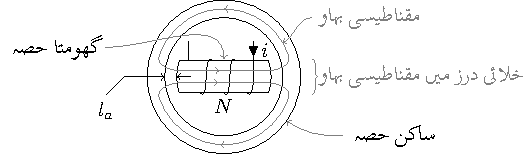
\includegraphics{figMagneticCircuitsSimpleRotatingMachineOutline}
\begin{tikzpicture}
\pgfmathsetmacro{\radI}{1} 
\pgfmathsetmacro{\radO}{1.3} 
\pgfmathsetmacro{\radAv}{(\radI+\radO)/2}
\pgfmathsetmacro{\rad}{0.8} 
\pgfmathsetmacro{\delTheta}{20} 
\pgfmathsetmacro{\yUP}{\rad*cos(\delTheta) } 
%machine stator dimensions
\draw (0,0) circle (\radI);
\draw (0,0) circle (\radO);

%==================================================
%the scope has been added to rotate everything by 35 degrees
%\begin{scope}[rotate=35]
%rotor at zero degrees
\draw (0,0)++(-\delTheta:\rad) arc (-\delTheta:\delTheta:\rad)--(180-\delTheta:\rad) arc (180-\delTheta:180+\delTheta:\rad)--cycle;
%winding on rotor
\foreach \x in {0.2,-0.2}
{
\draw (\x,0.28) to [out=135,in=-45]  (\x-0.2,-0.28);
}
%winding end connections
\draw(0.4,-0.28) to [out=-45,in=-90] (0.5,0) to (0.5,0.3) to [short,i_<=$i$](0.5,0.6);
\draw(-0.6,0.28) --(-0.6,0.6);
\draw(0,-0.5)node{$N$};
%flux upper half
\draw[gray](0.9*\delTheta:\radAv) to [out=-70,in=0] (0.4*\delTheta:0.9*\rad);
\draw[gray,-<-=0.6] (0.4*\delTheta:0.9*\rad)--(180-0.4*\delTheta:0.9*\rad);
\draw[gray](180-0.4*\delTheta:0.9*\rad) to [out=180,in=-110] (180-0.9*\delTheta:\radAv);
\draw[gray,->-=0.5](0.9*\delTheta:\radAv) arc (0.9*\delTheta:180-0.9*\delTheta:\radAv);
%flux lower half
\begin{scope}[rotate=180]
%
\draw[gray](0.9*\delTheta:\radAv) to [out=-70,in=0] (0.4*\delTheta:0.9*\rad);
\draw[gray,->-=0.43] (0.4*\delTheta:0.9*\rad)--(180-0.4*\delTheta:0.9*\rad);
\draw[gray](180-0.4*\delTheta:0.9*\rad) to [out=180,in=-110] (180-0.9*\delTheta:\radAv);
\draw[gray,-<-=0.5](0.9*\delTheta:\radAv) arc (0.9*\delTheta:180-0.9*\delTheta:\radAv);
\end{scope}
%urdu
\draw[gray,<-](-35:\radO) to [out=-35,in=180] (2,-1)node[black][right]{\RL{ساکن حصہ }};
\draw[gray,<-](0,0.3) to [out=90,in=0] (-2,0.5) node[left,black]{\RL{گھومتا حصہ}};
%
\draw[gray,decorate,decoration={brace,mirror}]  (1.5,-0.3) -- node[right] {\RL{خلائی درز میں مقناطیسی بہاو}} (1.5,0.3);
\draw[gray,<-] (30:\radAv) to [out=30,in=180] (1.5,1)node[right]{\RL{مقناطیسی بہاو}};
\draw[->] (180:0.7*\rad)--(180:\rad);
\draw[<-](180:\radI)--(180:1.3*\radO)--++(-0.3,-0.3)node[below]{$l_a$};
%\end{scope}
%===========================================
\end{tikzpicture}%

\caption{سادہ گھومنے والا مشین}
\label{شکل_مقناطیسی_دور_سادہ_گھومتا_مشین}
\end{figure}

حل:\quad
اس شکل میں گھومتے مشین، مثلاً موٹر، کی ایک سادہ صورت دکھائی گئی ہے۔ ایسی مشینوں کا بیرونی حصہ ساکن رہتا ہے لہٰذا اس حصے  کو مشین کا \اصطلاح{ساکن حصہ}\فرہنگ{ساکن حصہ}\حاشیہب{stator}\فرہنگ{stator} کہتے ہیں۔ساکن حصے کے اندر مشین کا  گھومتا حصہ پایا جاتا ہے لہٰذا اس حصے کو مشین کا \اصطلاح{گھومتا حصہ}\فرہنگ{گھومتا حصہ}\حاشیہب{rotor}\فرہنگ{rotor} کہتے ہیں۔ اس مثال میں ان دونوں حصوں کا  \عددیء{\mu_r=\infty}  ہے لہٰذا ان کی ہچکچاہٹ صفر ہو گی۔ مقناطیسی بہاو  کو ہلکی سیاہی کی لکیر سے ظاہر کیا گیا ہے۔ مقناطیسی بہاو کی ایک مکمل چکر کے دوران مقناطیسی بہاو دو خلائی درزوں  سے گزرتا ہے۔ یہ دو خلائی درز ہر لحاظ سے ایک جیسے ہیں لہٰذا ان دونوں خلائی درز کی ہچکچاہٹ بھی ایک دوسرے کے برابر ہوں گی۔مزید دونوں خلائی درزوں کی ہچکچاہٹ سلسلہ وار ہیں۔شکل \حوالہ{شکل_مقناطیسی_دور_سادہ_گھومتا_مشین} میں مقناطیسی بہاو کو گھومتے حصہ، ساکن حصہ اور دو خلائی درزوں  سے گزرتا ہوا دکھایا گیا ہے۔خلائی درز کی لمبائی \عددیء{l_a} بہت کم ہے لہٰذا خلائی درز کا عمودی رقبہ تراش \عددیء{A_a} وہی ہو گا جو گھومتے حصہ کا ہے یعنی \عددیء{A_a=A_c} ہو گا۔

ایک خلائی درز کی ہچکچاہٹ
\begin{align*}
\Re_a=\frac{l_a}{\mu_0 A_a}=\frac{l_a}{\mu_0 \A_c}
\end{align*}
ہے لہٰذا دو سلسلہ وار خلائی درزوں کی کُل ہچکچاہٹ درج ذیل ہو گی۔
\begin{align*}
\Re_s=\Re_a=\Re_a=\frac{2 l_a}{\mu_0 A_c}
\end{align*}
خلائی درز میں مقناطیسی بہاو \عددیء{\phi_a} اور کثافتِ مقناطیسی بہاو \عددیء{B_a} درج ذیل ہوں گے۔
\begin{align*}
\phi_a&=\frac{\tau}{\Re_s}=\left(N i \right) \left (\frac{\mu_0 A_c}{2 l_a} \right)\\
B_a&=\frac{\phi_a}{A_a}=\frac{\mu_0 N i}{2 l_a}
\end{align*}
اس مساوات میں اعداد استعمال کرتے ہیں۔
\begin{align*}
0.95&=\frac{4 \pi 10^{-7} \times 1000 \times i}{2 \times 0.005}\\
i&=\frac{0.95 \times 2 \times 0.005}{ 4 \pi 10^{-7} \times 1000}=\SI{7.56}{\ampere}
\end{align*}
موٹر اور جنریٹروں کی خلاء میں تقریباً ایک ٹسلا کثافتِ برقی بہاو ہوتی ہے۔
\انتہا{مثال}

\حصہ{خود امالہ  ، مشترکہ امالہ  اور توانائی}
مقناطیسی بہاو کی وقت کے ساتھ تبدیلی برقی دباو  کو جنم دیتی ہے۔ لہٰذا شکل \حوالہ{شکل_مقناطیسی_بہاو_تبدیلی_اور_دباو}-ا  کے قالب میں مقناطیسی بہاو \عددی{\phi} کی تبدیل کی بنا لچھے میں برقی دباو \عددی{e} پیدا ہو گا جو لچھے کے سروں پر نمودار ہو گا۔ اِس طرح پیدا ہونے والی برقی دباو کو \اصطلاح{امالی برقی دباو}\فرہنگ{امالی برقی دباو}\حاشیہب{induced voltage}\فرہنگ{induced voltage}  کہتے ہیں۔ \اصطلاح{قانونِ فیراڈے}\فرہنگ{فیراڈے!قانون}\حاشیہب{Faraday's law}\فرہنگ{Faraday's law}  کے تحت\حاشیہد{مائکل فیراڈے انگلستانی سائنسدان تھے جنہوں نے محرک برقی دباو دریافت کی}  درج ذیل ہو گا۔
\begin{align}\label{مساوات_مقناطیسی_دور_فیراڈے_قانون}
e=N \frac{\partial \phi}{\partial t} =\frac{\partial \lambda}{\partial t}
\end{align}
%
\begin{figure}
\centering
\begin{subfigure}{0.45\textwidth}
\centering
\begin{circuitikz}
\def\height{2};
\def\width{1.5};
\def\thick{0.4};
\def\depthX{0.2};
\def\depthY{0.2};
\def\gap{0.05};
%flux
\draw[gray,latex-](\width-\thick/2,1.8-0.25) to [out=120,in=0](\width/2,1.8)node[fill=white,black]{$\phi$} to [out=180,in=70](\thick/2,1.8-0.25);
%going clockwise from origin
\draw(0,0)--++(0,\height)--++(\width,0)--++(0,-\height)--cycle;
\draw(0,0)++(\thick,\thick)--++(0,\height-2*\thick)--++(\width-2*\thick,0)--++(0,-\height+2*\thick)--cycle;
%
\draw(\thick,\thick)--++(\depthX,\depthY) --++(0,\height-2*\thick-\depthY);
\draw(\thick,\thick)--++(\depthX,\depthY) --++(\width-2*\thick-\depthX,0);
\draw(0,\height)--++(\depthX,\depthY)--++(\width,0)--++(-\depthX,-\depthY);
\draw(\width,0)--++(\depthX,\depthY)--++(0,\height)--++(-\depthX,-\depthY);
%\draw[gray,-latex](\width/2,1.8)node[black]{$\phi$}++(-0.3,0) to [out=180,in=70]++(-0.25,-0.25);
%winding
\draw (0.6,1.4) to [out=45,in=0] (0.2,1.5) to [short] (-1,1.5) node[left]{$+$};
\foreach \l in {1.4,1.2,1}{
\draw (0,\l) to [out=-135,in=45] (0.6,\l-0.2);
}
\draw (0,0.8) to (-1,0.8)node[left]{$-$};
\node at (-1,1.15)[left]{$e$};
\draw($(0,1.5)!0.5!(0,0.8)$)node[left]{$N$};
\end{circuitikz}%
\caption{}
\end{subfigure}\hfill
\begin{subfigure}{0.45\textwidth}
\centering
\begin{circuitikz}
\def\height{2};
\def\width{1.5};
\def\thick{0.4};
\def\depthX{0.2};
\def\depthY{0.2};
\def\gap{0.05};
%flux
\draw[gray,-latex](\width-\thick/2,1.8-0.25) to [out=120,in=0](\width/2,1.8)node[fill=white,black]{$\phi'$} to [out=180,in=70](\thick/2,1.8-0.25);
%going clockwise from origin
\draw(0,0)--++(0,\height)--++(\width,0)--++(0,-\height)--cycle;
\draw(0,0)++(\thick,\thick)--++(0,\height-2*\thick)--++(\width-2*\thick,0)--++(0,-\height+2*\thick)--cycle;
%
\draw(\thick,\thick)--++(\depthX,\depthY) --++(0,\height-2*\thick-\depthY);
\draw(\thick,\thick)--++(\depthX,\depthY) --++(\width-2*\thick-\depthX,0);
\draw(0,\height)--++(\depthX,\depthY)--++(\width,0)--++(-\depthX,-\depthY);
\draw(\width,0)--++(\depthX,\depthY)--++(0,\height)--++(-\depthX,-\depthY);
%\draw[gray,-latex](\width/2,1.8)node[black]{$\phi$}++(-0.3,0) to [out=180,in=70]++(-0.25,-0.25);
%winding
\draw (0.6,1.4) to [out=45,in=0] (0.2,1.5) to [short] (-1,1.5)coordinate(kT) node[left]{$+$};
\foreach \l in {1.4,1.2,1}{
\draw (0,\l) to [out=-135,in=45] (0.6,\l-0.2);
}
\draw (0,0.8) to (-1,0.8)coordinate(kB)node[left]{$-$};
\draw(kT)to [short]++(0,0.5)--++(-1,0) to [resistor,i>_={$i$}]++(0,-2)-|(kB);
\node at (-1,1.15)[left]{$e$};
\draw($(0,1.5)!0.5!(0,0.8)$)node[left]{$N$};
\end{circuitikz}%
\caption{}
\end{subfigure}%
\caption{قالب میں مقناطیسی بہاو میں تبدیلی لچھے میں برقی دباو پیدا کرتی ہے۔}
\label{شکل_مقناطیسی_بہاو_تبدیلی_اور_دباو}
\end{figure}

امالی برقی دباو کو منبع برقی دباو تصور کریں۔

 امالی برقی دباو  کی سمت کا تعین یوں کیا جاتا ہے کہ اگر دیئے گئے لچھے کی سروں کو \اصطلاح{کسرِ دور}\فرہنگ{کسر دور}\حاشیہب{short circuit}   کیا جائے تو اِس میں برقی رو اُس رخ  ہو گی جو مقناطیسی بہاو کی تبدیلی کو روکے۔ یوں اگر شکل \حوالہ{شکل_مقناطیسی_بہاو_تبدیلی_اور_دباو}-ا میں بہاو کی سمت گھڑی کی سوئیوں کے گھومنے کے رخ ہو  اور اگر بہاو بڑھ رہا ہو تب بہاو کی تبدیلی کے مخالف بہاو پیدا کرنے کی خاطر لچھے کا بالائی سر مثبت دباو پر ہو گا۔شکل \حوالہ{شکل_مقناطیسی_بہاو_تبدیلی_اور_دباو}-ب میں لچھے کے سروں کے بیچ مزاحمت نسب کیا گیا ہے۔ لچھے کو منبع دباو تصور کرتے ہوئے  آپ دیکھ سکتے ہیں کہ مزاحمت میں رو کی سمت قالب میں گھڑی کی الٹ رخ بہاو \عددی{\phi'} پیدا کرے گا۔

قالب میں مقناطیسی بہاو \عددیء{\phi} لچھے کے تمام چکروں کے اندر سے گزرتا ہے۔\عددیء{N \phi} کو لچھے کی \اصطلاح{ارتباط بہاو}\فرہنگ{ارتباط بہاو}\حاشیہب{flux linkage} \عددیء{\lambda}  کہتے ہیں جس کی اکائی \اصطلاح{ویبر-چکر}\فرہنگ{ویبر-چکر}\حاشیہب{weber-turn}  ہے۔
\begin{align}
\lambda=N\phi
\end{align}
جن مقناطیسی ادوار میں مقناطیسی مستقل \عددیء{\mu}  کو اٹل مقدار تصور کیا جا سکے یا جن میں خلائی درز کی ہچکچاہٹ قالب کی ہچکچاہٹ سے بہت زیادہ ہو \عددیء{\Re_a \gg \Re_c}  ان میں لچھے کی  \اصطلاح{امالہ}\فرہنگ{امالہ}\حاشیہب{inductance}\فرہنگ{inductance} \عددیء{L}  کی تعریف درج ذیل ہے۔
\begin{align}\label{مساوات_مقناطیسی_دور_خود_امالہ_تعریف}
L=\frac{\lambda}{i}
\end{align}

امالہ کی اکائی ویبر-چکر فی ایمپیئر ہے جس کو \اصطلاح{ہینری}\فرہنگ{Henry}\حاشیہب{Henry}\فرہنگ{Henry} \عددیء{H} کا نام\حاشیہد{امریکی سائنسدان جوزف ہینری جنہوں نے مائکل فیراڈے سے علیحدہ  طور پر محرک برقی دباو دریافت کی} دیا گیا ہے۔ یوں \عددی{\lambda=N\phi}،  \عددی{\phi=B_cA_c}  اور \عددی{\phi=\tfrac{Ni}{\Re}} پر کرتے ہوئے درج ذیل حاصل ہوتا ہے
\begin{align}
L=\frac{N \phi}{i}=\frac{N B_c A_c}{i}=\frac{N^2 \mu_0 A_a}{l_a}
\end{align}
جہاں قالب کا رقبہ عمودی تراش \عددی{A_c} اور درز کا رقبہ عمودی تراش \عددی{A_a} ایک دوسرے کے برابر لیے گئے ہیں۔
%
\ابتدا{مثال}\شناخت{مثال_مقناطیسی_امالہ_الف}
شکل \حوالہ{شکل_مثال_مقناطیسی_امالہ_الف} میں \عددیء{b=\SI{5}{\centi \meter},w=\SI{4}{\centi\meter},l_a=\SI{3}{\milli \meter}} جبکہ لچھے کے \عددیء{1000} چکر اور قالب کی اوسط لمبائی \عددیء{l_c=\SI{30}{\centi\meter}} ہے۔درج ذیل دو صورتوں میں لچھے کی امالہ تلاش کریں۔
\begin{itemize}
\item
قالب کی \عددیء{\mu_r = \infty} ہے۔
\item
قالب کی \عددیء{\mu_r = 500} ہے۔
\end{itemize}
%
\begin{figure}
\centering
\begin{tikzpicture}
\def\height{2};
\def\width{1.5};
\def\thick{0.4};
\def\depthX{0.2};
\def\depthY{0.2};
\def\gap{0.05};
\pgfmathsetmacro{\widthX}{0.25}  
\pgfmathsetmacro{\widthY}{0.25}  
\coordinate(O) at (-0.5,0);
%grid
%\draw[gray,thick](0,0) grid (12,3);
%\draw[gray,thin,xstep=0.1,ystep=0.1](0,0) grid (12,3);
%going clockwise from origin
\draw(0,0)--++(0,\height)--++(\width,0)--++(0,-0.5*\height+\gap)--++(-\thick,0)--++(0,0.5*\height-\gap-\thick)--++(-\width+2*\thick,0)--++(0,-\height+2*\thick)--++(\width-2*\thick,0)--++(0,0.5*\height-\thick-\gap)--++(\thick,0)--++(0,-0.5*\height+\gap)--cycle;
%
\draw(\thick,\thick)--++(\depthX,\depthY) --++(0,\height-2*\thick-\depthY);
\draw(0.4,0.4)--++(\width-2*\thick-\depthX,0);
\draw(0,\height)--++(\depthX,\depthY)--++(\width,0)--++(-\depthX,-\depthY);
\draw(\width,\height)++(\depthX,\depthY)--++(0,-0.5*\height+\gap)--++(-\depthX,-\depthY);
\draw(\width,0)--++(\depthX,\depthY)--++(0,0.5*\height-\gap)--++(-\depthX,-\depthY);
\draw(\thick+\depthX,\thick+\depthY)--++(\width-2*\thick-\depthX,0);
%gap
\draw(1.7,1.155)--++(-0.1,0);
\draw(1.1,0.95)--++(0.1,0.1);
%winding
\draw (0.6,1.4) to [out=45,in=0] (0.2,1.5) to [short,i_<=$i$] (-1,1.5) node[left]{$+$};
\foreach \l in {1.4,1.2,1}{
\draw (0,\l) to [out=-135,in=45] (0.6,\l-0.2);
}
\draw (0,0.8) to (-1,0.8)node[left]{$-$};
%turns
\node at (0,1.15)[left]{$\tau=N i$};
%gap
\draw[gray](1.8,1.15)--++(0.3,0);
\draw[gray](1.8,1.25)--++(0.3,0);
\draw[->](2.2,1.7)node[right]{$l_a$}--++(-0.2,-0.2)--++(0,-0.25);
\draw[->](2,1)--++(0,0.15);
%flux
\draw[-latex,gray](1.1,1.8)node[left,black]{$\phi$}--++(0.2,0)--++(0,-\height+\thick)--++(-\width+\thick,0)--++(0,\height-\thick)--++(0.5,0);
%dimensions
\draw[,<->] (1.1,-0.1)--++(0.4,0)node[below,pos=0.5]{$b$};
\draw[<->](1.5+0.1,-0.1)--++(0.2,0.2)node [pos=0.4,right]{$w$};
\end{tikzpicture}%
\caption{امالہ (مثال \حوالہ{مثال_مقناطیسی_امالہ_الف})}
\label{شکل_مثال_مقناطیسی_امالہ_الف}
\end{figure}

حل:\quad
(ا) \quad 
 قالب کی \عددیء{\mu_r=\infty}  کی بنا قالب کی ہچکچاہٹ نظرانداز کی جا سکتی ہے۔یوں امالہ درج ذیل ہو گی۔
\begin{align*}
L&=\frac{N^2 \mu_0 w b}{l_a}\\
&=\frac{1000^2 \times 4 \pi 10^{-7} \times 0.04 \times 0.05}{0.003}\\
&=\SI{0.838}{\henry}
\end{align*}
(ب) \quad
 \عددیء{\mu_r=500} کی صورت میں قالب کی ہچکچاہٹ قابل نظر انداز نہیں ہو گی۔خلاء اور قالب کی ہچکچاہٹ  دریافت کرتے ہیں۔
\begin{align*}
\Re_a&=\frac{l_a}{\mu_0 w b}=\frac{0.003}{4\pi 10^{-7} \times 0.04 \times 0.05}=\SI{1193507}{\ampere \cdot t \per \weber}\\
\Re_c&=\frac{l_c}{\mu_r \mu_0 w b}=\frac{0.3}{500 \times 4\pi 10^{-7} \times 0.04 \times 0.05}=\SI{238701}{\ampere \cdot t \per \weber}
\end{align*}
یوں درج ذیل ہو گا۔
\begin{align*}
\phi&=\frac{N i}{\Re_a+\Re_c}\\
\lambda &= N \phi = \frac{N^2 i}{\Re_a+\Re_c}\\
L&=\frac{\lambda}{i}=\frac{N^2}{\Re_a+\Re_c}=\frac{1000^2}{\num{1193507}+\num{238701}}=\SI{0.698}{\henry}
\end{align*}
\انتہا{مثال}
%
\ابتدا{مثال}
شکل \حوالہ{شکل_مقناطیسی_ادوار_پیچدار_لچھا} میں ایک پیچدار لچھا\فرہنگ{لچھا!پیچدار}\حاشیہب{spiral coil} دکھایا گیا ہے جس کی جسامت درج ذیل ہے۔
\begin{align*}
\عددیء{N=11, r=\SI{0.49}{\meter},l=\SI{0.94}{\meter}}
\end{align*}
پیچدار لچھے  کے اندر مقناطیسی بہاو \عددی{\phi} کا بیشتر حصہ محوری رخ ہوتا ہے۔ لچھے کے بار یہی بہاو پوری کائنات سے گزرتے ہوئے واپس لچھے میں داخل ہوتا ہے۔چونکہ پوری کائنات کا رقبہ عمودی تراش \عددی{A} لامتناہی ہے لہٰذا لچھے کے باہر کثافت مقناطیسی بہاو \عددی{B=\tfrac{\phi}{A}} کی مقدار قابل نظرانداز ہوتی ہے۔لچھے کے اندر محوری رخ مقناطیسی شدت درج ذیل ہو گی۔
\begin{align*}
H=\frac{N i}{l}
\end{align*}
اس لچھے کی خود امالہ حاصل کریں۔
\begin{figure}[h!]
\centering
\begin{tikzpicture}
\pgfmathsetmacro{\radX}{1.8}
 \pgfmathsetmacro{\radY}{0.4}
\pgfmathsetmacro{\thetaStart}{0} 
\pgfmathsetmacro{\thetaEnd}{180}
%grid
%\draw[gray,thick] (-4*\radX,-4*\radX) grid (4*\radX,4*\radX);
%\draw[gray,thin,xstep=0.1,ystep=0.1] (-4*\radX,-4*\radX) grid (4*\radX,4*\radX);
%coil backside
\foreach \y in {0,0.2,0.4,0.6,0.8,1,1.2,1.4,1.6,1.8,2}{
\draw[thick,domain={0:180},variable=\t,smooth,samples=100] plot({\radX*cos(\t)},{\y+0.1/180*\t+\radY*sin(\t)});
}
%coil front
\foreach \y in {0,0.2,0.4,0.6,0.8,1,1.2,1.4,1.6,1.8,2}{
\draw[thick,domain={180:360},variable=\t,smooth,samples=100] plot({\radX*cos(\t)},{\y+0.1/180*\t+\radY*sin(\t)});
}
%end connections
\draw[thick](\radX,0)--(1.4*\radX,0);
\draw[thick](\radX,2+0.1/180*360)--(1.4*\radX,2+0.1/180*360);
%text
\draw[gray,<->](1.4*\radX,0+0.05)--(1.4*\radX,2+0.1/180*360-0.05)node[pos=0.5,right]{$l$};
\draw[gray,dashed](0,2+0.1/180*360-0.4)--(0,2+0.1/180*360+0.4);
\draw[gray,->] (0,2+0.1/180*360+0.4)--++(\radX,0)node [above,pos=0.5]{$r$};
\draw(-2,1)node[left]{\RL{$N$ چکر}};
\end{tikzpicture}
\caption{پیچدار لچھا}
\label{شکل_مقناطیسی_ادوار_پیچدار_لچھا}
\end{figure}

حل:
\begin{align*}
B&=\mu_0 H=\frac{\mu_0 N i}{l}\\
\phi&=B  \pi r^2=\frac{\mu_0 N i \pi r^2}{l}\\ 
\lambda&=N \phi =\frac{\mu_0 N^2 i \pi r^2}{l}\\ 
L&=\frac{\lambda}{i}=\frac{\mu_0 N^2 \pi r^2}{l}
\end{align*} 
عددی{N}، \عددی{r} اور \عددی{l} کی قیمتیں پر کرتے ہوئے درج ذیل امالہ حاصل ہو گا\حاشیہد{یہ پیچدار لچھا میں نے  \عددی{3000} کلو گرام لوہا پگھلانے والی بھٹی میں استعمال کیا ہے۔}۔
\begin{align*}
L=\frac{4 \pi 10^{-7} \times 11^2 \times \pi  \times 0.49^2}{0.94}=\SI{122}{\micro \henry}
\end{align*}
\انتہا{مثال}
%
شکل \حوالہ{شکل_مقناطیسی_ادوار_دو_لچھے_ایک_درز} میں دو لچھے والا ایک مقناطیسی دور دکھایا گیا ہے۔ ایک لچھے کے چکر  \عددیء{N_1}  اور اس میں برقی رو \عددیء{i_1} ہے،  دوسرا لچھا \عددیء{N_2} چکر کا ہے اور اس میں برقی  رو \عددیء{i_2} ہے۔ دونوں لچھوں میں مثبت برقی رو قالب میں ایک جیسے  رخ  مقناطیسی دباو  پیدا کرتے ہیں۔ اگر قالب کا \عددی{\Re_c} قابل نظرانداز ہو تب مقناطیسی بہاو \عددیء{\phi}درج ذیل ہو گا۔
\begin{align}
\phi=\left (N_1 i_1 +N_2 i_2 \right ) \frac{\mu_0 A_a}{l_a}
\end{align} 
%
\begin{figure}[h!]
\centering
\begin{tikzpicture}
%grid
%\draw[gray,thick] (0,0) grid (12,2);
%\draw[gray,thin,xstep=0.1,ystep=0.1] (0,0) grid (12,2);
\def\h{2}
\def\w{2.4}
\def\t{0.4}
\def\g{0.2}
%core
\draw (0,0)--++(0,\h)--++(\w/2-\g/2,0)--++(0,-\t)--++(-\w/2+\g/2+\t,0)--++(0,-\h+\t+\t)--++(\w-\t-\t,0)--++(0,\h-\t-\t)--++(-\w/2+\t+\g/2,0)--++(0,\t)--++(\w/2-\g/2,0)--++(0,-\h)--cycle;
%flux
\draw[gray,->-=0.86](\t/2,\t/2)--++(0,\h-\t)--++(\w-\t,0)--++(0,-\h+\t)--cycle;
%left hand coils
\foreach \y in {0.7,0.9,1.1,1.3}{
\draw (0,\y) to [out=-135,in=45](0.4,\y-0.1);
}
%end connection
\draw (0.4,1.4) to [out=45,in=0] (0.2,1.45);
\draw(0.2,1.45) to ++(-0.3,0) to [short,i_<=$i_1$] ++(-0.3,0);
\draw (0,0.5)--++(-0.4,0);
%right hand coils
\foreach \y in {0.7,0.9,1.1,1.3}{
\draw (\w,\y) to [out=-45,in=135](\w-\t,\y-0.1);
}
%end connection
\draw (\w-\t,1.4) to [out=135,in=0] (\w-\t/2,1.45);
\draw(\w-\t/2,1.45) to ++(0.3,0) to [short,i<=$i_2$] ++(0.3,0);
\draw (\w,0.5)--++(0.4,0);
%text
\draw(\t,\h/2) node[right]{$N_1$};
\draw(\w-\t,\h/2) node[left]{$N_2$};
\draw(0,\h/2) node[left]{$\lambda_1$};
\draw(\w,\h/2) node[right]{$\lambda_2$};
%gap
\draw (\w/2-\g/2,\h+0.1)--++(0,0.2);
\draw (\w/2+\g/2,\h+0.1)--++(0,0.2);
\draw[->](\w/2-\g/2-0.2,\h+0.2)--++(0.2,0);
\draw[<-](\w/2+\g/2,\h+0.2)--++(0.2,0)--++(0.1,0.1)node[above right]{$l_a$};
\draw[->](\t+0.2,\h-\t-0.2)--++(0,0.2);
\draw[<-](\t+0.2,\h)--++(0,0.2)--++(-0.1,0.1)node[above left]{$b$};
%equations
\draw (6.5,\h/2) node[right]{$
\begin{aligned}
A_a&=A_c=b w\\
\lambda_1&=N_1 \phi\\
\lambda_2&=N_2 \phi\\
\phi&=\frac{N_1 i_1 + N_2 i_2}{\Re_a+\Re_c}
\end{aligned}
$};
%urdu
\draw (4,\h/2) node[above right]{موٹائی $=b$};
\draw(4,\h/2) node[below right]{ گہرائی $=w$};
\end{tikzpicture}%

\caption{دو لچھے والا مقناطیسی دور۔}
\label{شکل_مقناطیسی_ادوار_دو_لچھے_ایک_درز}
\end{figure}
دونوں لچھوں کے مجموعی مقناطیسی دباو یعنی \عددیء{N_1 i_1+N_2 i_2} سے پیدا ہونے والا مقناطیسی بہاو \عددیء{\phi}  ہے۔ اس مقناطیسی بہاو  کا پہلے  لچھے  کے ساتھ  ارتباط
\begin{align}
\lambda_1=N_1 \phi=N_1^2  \frac{\mu_0 A_a}{l_a} i_1 +N_1 N_2  \frac{\mu_0 A_a}{l_a} i_2
\end{align}
یعنی
\begin{align}\label{مساوات_مقناطیسی_دور_ارتباط_دو_لچھے}
\lambda_1 = L_{11} i_1+L_{12} i_2
\end{align}
ہے جہاں \عددی{L_{11}} اور \عددی{L_{12}} سے مراد درج ذیل ہے۔
\begin{align}
L_{11}&=N_1^2  \frac{\mu_0 A_a}{l_a}\\
L_{12}&=N_1 N_2  \frac{\mu_0 A_a}{l_a}
\end{align}
\عددیء{L_{11}} پہلے لچھے کی  \اصطلاح{خود امالہ}\فرہنگ{خود امالہ}\حاشیہب{self inductance}\فرہنگ{self inductance}  ہے اور  \عددیء{L_{11} i_1} اس لچھے کی اپنے برقی رو \عددیء{i_1} سے پیدا مقناطیسی بہاو  کے ساتھ  ارتباط بہاو ہے جسے \اصطلاح{خود ارتباط بہاو}\فرہنگ{خود ارتباط بہاو}\حاشیہب{self flux linkage}\فرہنگ{self flux linkage} کہتے ہیں۔\عددیء{L_{12}}  اِن دونوں لچھوں  کا  \اصطلاح{مشترکہ امالہ}\فرہنگ{مشترکہ امالہ}\حاشیہب{mutual inductance}\فرہنگ{mutual inductance} ہے اور  \عددیء{L_{12} i_2}  لچھا-1  کے ساتھ  \عددیء{i_2} سے پیدا بہاو کے ساتھ  ارتباط بہاو  ہے جسے \اصطلاح{مشترکہ ارتباط بہاو}\فرہنگ{مشترکہ ارتباط امالہ}\حاشیہب{mutual flux linkage}\فرہنگ{mutual flux linkage}  کہتے ہیں ۔ بالکل اسی طرح ہم دوسرے لچھے کے لئے درج ذیل لکھ سکتے ہیں
\begin{align}
\lambda_2&=N_2 \phi=N_2 N_1 \frac{\mu_0 A_a}{l_a} i_1+N_2^2 \frac{\mu_0 A_a}{l_a} i_2  \nonumber \\
&=L_{21} i_1+L_{22} i_2 \label{مساوات_مقناطیسی_دور_دوسرے_لچھے_کی_ارتباط}
\end{align}
جہاں \عددی{L_{22}} اور \عددی{L_{21}} سے مراد درج ذیل ہے۔
\begin{align}
L_{22}&=N_2^2 \frac{\mu_0 A_a}{l_a}\\
L_{21}&=L_{12}=N_2 N_1 \frac{\mu_0 A_a}{l_a} \label{مساوات_مقناطیسی_دور_مشترکہ_امالہ_یکساں}
\end{align}
\عددیء{L_{22}} لچھا-2  کی خود امالہ اور  \عددیء{L_{21}=L_{12}} دونوں لچھوں کی مشترکہ امالہ ہے۔امالہ کا تصور اس وقت کارآمد ہوتا ہے جب مقناطیسی مستقل \عددیء{\mu}  کو اٹل تصور کرنا ممکن ہو۔

مساوات \حوالہ{مساوات_مقناطیسی_دور_خود_امالہ_تعریف}  کو مساوات \حوالہ{مساوات_مقناطیسی_دور_فیراڈے_قانون}  میں پر کرتے ہیں۔
\begin{align}
e=\frac{\partial \lambda}{\partial t}=\frac{\partial \left( L i\right) }{\partial t}
\end{align}
اگر امالہ کی قیمت اٹل ہو جیسا کہ ساکن مشینوں  میں ہوتا ہے تب ہمیں  امالہ کی جانی پہچانی مساوات
\begin{align}
e=L \frac{\partial i}{\partial t}
\end{align}
ملتی ہے۔ اگر امالہ بھی تبدیل ہو جیسا کہ موٹروں اور جنریٹروں میں ہوتا ہے تب درج ذیل ہو گا۔
\begin{align}
e= L \frac{\partial i}{\partial t} + i \frac{\partial L}{\partial t}
\end{align}

\اصطلاح{توانائی}\فرہنگ{توانائی}\حاشیہب{energy}\فرہنگ{energy}  کی اکائی \اصطلاح{جاول}\فرہنگ{جاول}\حاشیہب{Joule}\فرہنگ{Joule} \عددیء{J}\حاشیہد{جیمس پریسقوٹ جاول انگلستانی سائنسدان جنہوں نے حرارت اور میکانی کام کا رشتہ دریافت کیا} ہے اور \اصطلاح{طاقت}\فرہنگ{طاقت}\حاشیہب{power}\فرہنگ{power}  کی اکائی\حاشیہد{سکاٹلینڈ کے جیمز واٹ جنہوں نے بخارات پر چلنے والے انجن پر کام کیا} جاول فی سیکنڈ یا \اصطلاح{واٹ}\فرہنگ{واٹ}\حاشیہب{Watt}\فرہنگ{Watt} \عددیء{W}  ہے۔

اس کتاب میں توانائی یا کام کو \عددیء{W} سے ظاہر کیا جائے لیکن طاقت کی اکائی واٹ \عددیء{W} کے لئے بھی یہی علامت استعمال ہوتی ہے۔امید کی جاتی ہے کہ متن سے  اصل مطلب جاننا ممکن ہو گا۔

وقت کے ساتھ توانائی کی تبدیلی کی شرح کو \اصطلاح{طاقت} کہتے ہیں۔اس طرح درج ذیل لکھا جا سکتا ہے۔
\begin{align}
p=\frac{\dif W}{\dif t} = ie = i \frac{\partial \lambda}{\partial t}
\end{align} 
مقناطیسی دور میں  لمحہ \عددیء{t_1} تا \عددیء{t_2}  مقناطیسی توانائی کی تبدیلی کو تکمل کے ذریعہ حاصل کیا جا سکتا ہے:
\begin{align}
\Delta W = \int_{t1}^{t2} p \dif t =\int_{\lambda1}^{\lambda2} i \dif \lambda
\end{align}
اگر مقناطیسی دور میں ایک ہی لچھا ہو اور دور میں امالہ کی قیمت اٹل ہو تب درج ذیل ہو گا۔
\begin{align}
\Delta W = \int_{\lambda1}^{\lambda2} i \dif \lambda=\int_{\lambda1}^{\lambda2} \frac{\lambda}{L} \dif \lambda=\frac{1}{2 L} \left(\lambda_2^2-\lambda_1^2 \right)
\end{align}

اگر لمحہ \عددیء{t_1} پر \عددیء{\lambda_1=0} تصور کیا جائے تب کسی دیئے گئے \عددیء{\lambda} پر مقناطیسی توانائی درج ذیل ہو گی۔
\begin{align}
\Delta W=\frac{\lambda^2}{2L}=\frac{L i^2}{2}
\end{align}

\حصہ{مقناطیسی مادہ کے خصوصیات}\شناخت{حصہ_مقناطیسی_دور_مقناطیسی_مادہ_کے_خصوصیات}
قالب کی استعمال سے دو فوائد حاصل ہوتے ہیں۔ قالب کے استعمال سے کم مقناطیسی دباو، زیادہ مقناطیسی بہاو پیدا کرتا ہے اور مقناطیسی بہاو کو پسند کی راہ پابند کیا جا سکتا ہے۔ ایک مرحلہ ٹرانسفارمروں میں قالب کی استعمال سے مقناطیسی بہاو کو یوں پابند کیا جاتا ہے کہ تمام لچھوں میں یکساں بہاو پایا جاتا ہو۔ موٹروں میں قالب کی استعمال سے مقناطیسی بہاو کو یوں پابند کیا جاتا ہے کہ زیادہ سے زیادہ قوت پیدا ہو جبکہ جنریٹروں میں زیادہ سے زیادہ برقی دباو حاصل کرنے کی نیت سے بہاو کو پابند کیا جاتا ہے۔
%==========
\begin{figure}
\centering
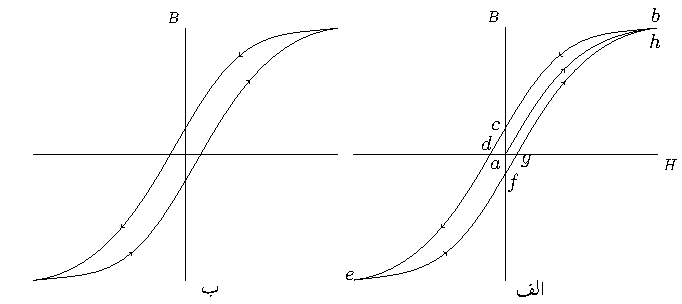
\includegraphics{figMagneticCircuitsBrillouinFunctionHysterisisLoop}
%\begin{tikzpicture}
%\draw(-1.5,0)--(1.5,0);
%\draw(0,-1.2)--(0,1.25);
%\draw(-1,-1).. controls (1,0) and (0,1)..(1,1);
%\end{tikzpicture}
\caption{$B-H$   خطوط یا مقناطیسی چال کے دائرے}
\label{شکل_مقناطیسی_چال}
\end{figure}
مقناطیسی اشیاء کی \عددیء{B} اور \عددیء{H} کے تعلق کو گراف کے ذریعہ سے پیش کیا جاتا ہے۔ لوہا نما مقناطیسی اشیاء کی \عددیء{B-H}  گراف شکل \حوالہ{شکل_مقناطیسی_چال}-الف میں دکھائی گئی ہے۔ایک لوہا نما مقناطیسی شہ جس میں کسی قسم کی مقناطیسی اثر نہ ہو کو نقطہ \عددیء{a} سے ظاہر کیا گیا ہے۔اس نقطہ پر
\begin{gather}
\begin{aligned}
H_a&=0\\
B_a&=0
\end{aligned}
\end{gather}
ہیں۔

	ایسی شہ کو لچھے میں رکھ کر اس پر مقناطیسی دباو لاگو کی جا سکتی ہے۔ مقناطیسی میدان کی شدت \عددیء{H}  لاگو کرنے سے لوہا نما مقناطیسی شہ میں کثافتِ مقناطیسی بہاو  \عددیء{B} پیدا ہو گی۔میدانی شدت بڑھانے سے کثافتِ مقناطیسی بہاو بھی بڑھے گی۔اس عمل کو نقطہ  \عددیء{a} سے شروع ایک نوکدار خط سے دکھلایا گیا ہے۔میدانی شدت کو نقطہ \عددیء{b}  تک بڑھایا گیا ہے جہاں یہ مقداریں  \عددیء{H_b} اور \عددیء{B_b} ہیں۔

	اگر اس نقطہ تک پہنچنے کے بعد میدانی شدت کم کی جائے تو دیکھا یہ گیا ہے کہ واپسی کی خط مختلف راستہ اختیار کرتی ہے۔یوں نقطہ  \عددیء{b} سے اگر میدانی شدت کم کرتے کرتے صفر کی جائے تو لوہا نما شہ کی کثافتِ مقناطیسی بہاو کم ہو کر نقطہ \عددیء{c} پر آ پہنچتی ہے۔نقطہ \عددیء{b} سے نقطہ \عددیء{c} تک نوکدار خط اس عمل کو دکھلا رہی ہے۔اس نقطہ پر بیرونی میدانی شدت صفر ہے لیکن لوہا نما شہ کی کثافتِ مقناطیسی بہاو صفر نہیں۔یہ اب ایک مقناطیس بن گیا ہے جس کی کثافتِ مقناطیسی بہاو  \عددیء{B_c} ہے۔اس مقدار کو \اصطلاح{بقایا کثافتِ مقناطیسی بہاو}\فرہنگ{کثافت مقناطیسی بہاو!بقایا}\حاشیہب{magnetic flux!residual}\فرہنگ{residual magnetic flux}  کہتے ہیں۔مصنوعی مقناطیس اسی طرح بنائے جاتے ہیں۔

اگر یہاں سے میدانی شدت منفی سمت میں بڑھائی جائے تو \عددیء{B} کم ہوتے ہوتے آخر کار ایک مرتبہ پھر صفر ہو جاتی ہے۔اس نقطہ کو \عددیء{d} سے ظاہر کیا گیا ہے۔مقناطیسیت ختم کرنے کے لئے درکار میدانی شدت کی مقدار  \عددیء{\abs{H_d}} کو مقناطیسیت ختم کرنے والی شدت یا \اصطلاح{خاتم شدت}\فرہنگ{مقناطیس!خاتم شدت}\حاشیہب{coercivity}\فرہنگ{coercivity} کہتے ہیں۔

منفی سمت میں میدانی شدت بڑھاتے نقطہ \عددیء{e} حاصل ہوتا ہے جہاں سے منفی سمت کی میدانی شدت کی مقدار ایک مرتبہ پھر کم کی جاتی ہے۔یوں نقطہ \عددیء{f} حاصل ہوتا ہے جہاں میدانی شدت صفر ہونے کے باوجود کثافتِ مقناطیسی بہاو صفر نہیں۔اس نقطہ پر لوہا نما شہ اُلٹ سمت میں مقناطیس بن چکا ہے اور \عددیء{B_f} بقایا کثافتِ مقناطیسی بہاو ہے۔اسی طرح اس جانب مقناطیسیت ختم کرنے کی شدت \عددیء{\abs{H_g}} ہے۔میدانی شدت بڑھاتے ہوئے ہم نقطہ \عددیء{b} کی بجائے نقطہ \عددیء{h} پہنچتے ہیں۔

اگر برقی شدت کو متواتر اسی طرح پہلے ایک جانب اور پھر دوسری جانب  ایک خاص حد تک لے جایا جائے تو آخر کار \عددیء{B-H}  خط ایک بند دائرے کی شکل اختیار کر لیتا ہے جسے شکل \حوالہ{شکل_مقناطیسی_چال}-ب میں دکھایا گیا ہے۔شکل \حوالہ{شکل_مقناطیسی_چال}-ب کو  \اصطلاح{مقناطیسی چال} کا دائرہ\فرہنگ{مقناطیس!چال کا دائرہ}\حاشیہب{hysteresis loop}\فرہنگ{hysteresis loop}  کہتے ہیں۔
\begin{figure}
\centering
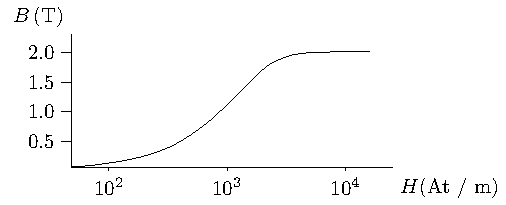
\includegraphics{figMagneticCircuitsM5curve}
\caption{$M5$ سٹیل کی $0.3048$ ملی میٹر موٹی پتری کا خط۔ میدانی شدت کا پیمانہ لاگ ہے۔}
\label{شکل_مقناطیسی_ادوار_ایم_پانچ_پتری_کا_خط}
\end{figure}

مختلف \عددیء{H} کے لئے  شکل \حوالہ{شکل_مقناطیسی_چال}-ب حاصل کر کے ایک ہی کاغذ پر کھینچنے کے بعد ان تمام کے  \عددیء{b} نقطے جوڑنے سے شکل \حوالہ{شکل_مقناطیسی_ادوار_ایم_پانچ_پتری_کا_خط} میں دکھایا \عددیء{B-H} خط حاصل ہوتا ہے۔ شکل \حوالہ{شکل_مقناطیسی_ادوار_ایم_پانچ_پتری_کا_خط} میں ٹرانسفارمروں میں استعمال ہونے والی  \عددیء{0.3048}  ملی میٹر موٹی \عددیء{M5} قالب کی پتری کا \عددیء{B-H} خط دکھایا گیا ہے۔ اس خط میں موجود مواد جدول \حوالہ{جدول_مقناطیسی_ادوار_کثافت_بہاو_بالمقابل_شدت}  میں بھی دیا گیا ہے۔عموماً مقناطیسی مسائل حل کرتے ہوئے شکل \حوالہ{شکل_مقناطیسی_چال} کی جگہ شکل \حوالہ{شکل_مقناطیسی_ادوار_ایم_پانچ_پتری_کا_خط} کی طرح کا خط استعمال کیا جاتا ہے۔دھیان رہے کہ اس خط میں \عددیء{H}  کا پیمانہ \اصطلاح{لاگ}\حاشیہب{log} میں دکھایا گیا ہے۔

لوہا نما مقناطیسی اشیاء پر لاگو مقناطیسی شدت بڑھانے سے کثافتِ مقناطیسی بہاو بڑھنے کی شرح بتدریج کم ہوتی جاتی ہے حتیٰ کہ آخر کار یہ شرح خلاء کی شرح  \عددیء{\mu_0} رہ جاتی ہے یعنی
\begin{align}
\frac{\Delta B}{\Delta H}=\mu_0
\end{align}
اس اثر کو \اصطلاح{سیرابیت}\فرہنگ{سیرابیت}\حاشیہب{saturation}\فرہنگ{saturation} کہتے ہیں۔یہ شکل \حوالہ{شکل_مقناطیسی_ادوار_ایم_پانچ_پتری_کا_خط}  میں واضح ہے۔

شکل \حوالہ{شکل_مقناطیسی_چال} سے واضح ہے کہ \عددیء{H} کے کسی بھی قیمت پر \عددیء{B} کے  دو ممکنہ قیمتیں ہیں۔ اگر مقناطیسی بہاو بڑھ رہا ہو تو گراف میں نیچے سے اُوپر جانے والی لکیر اِس میں \عددیء{B} اور \عددیء{H} کے تعلق کو پیش کرتی ہے اور اگر مقناطیسی بہاو کم ہو رہا ہو تو اوپر سے نیچے آنے والی لکیر اِس تعلق کو پیش کرتی ہے۔  چونکہ \عددیء{\mu=B/H} ، لہٰذا \عددیء{B} کے  مقدار تبدیل ہونے سے \عددیء{\mu} بھی تبدیل ہوتی ہے۔ باوجود اِس کے ہم مقناطیسی دوروں میں یہ تصور کرتے ہیں کہ \عددیء{\mu} ایک مقررہ ہے۔ یہ تصور کر لینے سے عموماً جواب پر زیادہ اثر نہیں پڑتا۔
%
\ابتدا{مثال}
شکل \حوالہ{شکل_مقناطیسی_ادوار_ایم_پانچ_پتری_کا_خط}  یا اس کے مساوی جدول \حوالہ{جدول_مقناطیسی_ادوار_کثافت_بہاو_بالمقابل_شدت} میں دیئے گئے مواد کو استعمال کرتے ہوئے شکل \حوالہ{شکل_مقناطیسی__کثافت_مقناطیسی_بہاو_اور_شدت}  کی خلاء میں ایک ٹسلا اور دو ٹسلا کثافتِ  مقناطیسی بہاو حاصل کرنے کے لئے درکار برقی رو معلوم کریں۔اس شکل میں
\begin{align*}
b=\SI{5}{\centi\meter},w=\SI{4}{\centi\meter},l_a=\SI{3}{\milli\meter},l_c=\SI{30}{\centi\meter},N=1000
\end{align*}
ہیں۔قالب اور خلاء کی رقبہ عمودی تراش برابر لیں۔

حل:\quad
 ایک ٹسلا کے لئے۔\\
 جدول \حوالہ{جدول_مقناطیسی_ادوار_کثافت_بہاو_بالمقابل_شدت}  سے ہم دیکھتے ہیں کہ قالب میں \عددیء{1} ٹسلا  حاصل کرنے کے لئے  قالب کو \عددیء{11.22}  ایمپیئر-چکر فی \عددیء{H} میٹر  درکار ہے۔یوں \عددیء{30} سم لمبے قالب کو \عددیء{0.3\times 11.22=3.366}  ایمپیئر چکر درکار ہیں۔

خلاء کو
\begin{align*}
H=\frac{B}{\mu_0}=\frac{1}{4\pi 10^{-7}}=\num{795671}
\end{align*}
ایمپیئر-چکر فی میٹر درکار ہیں۔لہٰذا \عددیء{ 3 } ملی میٹر لمبی خلاء کو \عددیء{0.003 \times 795671=2387} ایمپیئر چکر درکار ہیں۔یوں کُل ایمپیئر-چکر \عددیء{3.366+2387=2390.366} ہیں جن سے 
\begin{align*}
i=\frac{2390.366}{1000}=\SI{2.39}{\ampere}
\end{align*}	
حاصل ہوتی ہے۔

حل: دو ٹسلا کے لئے۔

جدول \حوالہ{جدول_مقناطیسی_ادوار_کثافت_بہاو_بالمقابل_شدت} سے ہم دیکھتے ہیں کہ قالب میں \عددیء{2} ٹسلا  حاصل کرنے کے لئے  قالب کو \عددیء{10000} ایمپیئر-چکر فی میٹر \عددیء{H} درکار ہے۔یوں \عددیء{30} سم لمبے قالب کو \عددیء{0.3 \times 10000=3000} ایمپیئر چکر درکار ہیں۔خلاء کو
\begin{align*}
H=\frac{B}{\mu_0}=\frac{2}{4\pi 10^{-7}}=\num{1591342}
\end{align*}
ایمپیئر-چکر فی میٹر درکار ہیں۔لہٰذا \عددیء{3} ملی میٹر لمبی خلاء کو  \عددیء{0.003 \times 1591342=4774}  ایمپیئر چکر درکار ہیں۔یوں کُل ایمپیئر-چکر \عددیء{3000+4774=7774}	ہیں جن سے 
\begin{align*}
i=\frac{7774}{1000}=\SI{7.774}{\ampere}
\end{align*}
حاصل ہوتی ہے۔

اس مثال میں مقناطیسی سیرابیت کے اثرات واضح ہیں۔ 
\انتہا{مثال}
%
\begin{table}
\begin{tabular}{l l l l   l l l l   l l l l}
$H$&$B$&$H$&$B$&$H$&$B$&$H$&$B$&$H$&$B$&$H$&$B$\\
\hline\\
9000&1.998&1000&1.852&           200&1.720 &30&1.480               &9&0.700&  0&0.000    \\
10000&2.000&2000&1.900&         300&1.752 &40&1.540           &10&0.835&  2&0.040    \\
20000&2.020&3000&1.936&         400&1.780 &50&1.580          &11.22&1.000&  3&0.095    \\
30000&2.040& 4000&1.952&        500&1.800 &60&1.601         &12.59&1.100 &  4&0.160    \\
40000&2.048&5000&1.968&         600&1.810 &70&1.626          &14.96&1.200&   5&0.240    \\
50000&2.060&6000&1.975&         700&1.824 &80&1.640         &17.78&1.300&  6&0.330    \\
60000&2.070&7000&1.980&         800&1.835  &90&1.655         &20&1.340&  7&0.440    \\
 70000&2.080&8000&1.985&        900&1.846 &100&1.662          &23.77&1.400& 8&0.560    \\
\hline
\end{tabular}
\caption{مقناطیسی بہاو بالمقابل شدت}
\label{جدول_مقناطیسی_ادوار_کثافت_بہاو_بالمقابل_شدت}
\end{table}
%

\حصہ{ہیجان شدہ لچھا}
عموماً بدلتی رو بجلی میں برقی دباو اور مقناطیسی بہاو سائن نما ہوتے ہیں یعنی یہ وقت کے ساتھ \عددیء{\sin \omega t} یا \عددیء{\cos \omega t} کا تعلق رکھتے ہیں۔ اِس سبق میں ہم بدلتی رو سے لچھے کو ہیجان کرنا اور اس سے نمودار ہونے والے برقی توانائی  کے ضیاع  کا تذکرہ  کریں گے۔ ہم فرض کرتے ہیں کہ قالب میں کثافتِ مقناطیسی بہاو 
\begin{align}
B=B_0 \sin \omega t
\end{align}
یوں قالب میں بدلتا مقناطیسی بہاو \عددیء{\varphi}
\begin{align}
\varphi=A_c B=A_c B_0 \sin \omega t=\phi_0 \sin \omega t
\end{align}
ہے۔اس مساوات میں مقناطیسی بہاو کا حیطہ  \عددیء{\mp\phi_0} اور \عددیء{B} کا حیطہ \عددیء{\mp B_0} کے مابین تبدیل ہوتے ہیں۔\عددیء{A_c} قالب کا رقبہ عمودی تراش ہے جو ہر جگہ یکساں ہے ۔\عددیء{\omega = 2 \pi f} ہے جہاں \عددیء{f} تعدد ہے۔

فیراڈے کے قانون یعنی مساوات \حوالہ{مساوات_مقناطیسی_دور_فیراڈے_قانون}  کے تحت اس مقناطیسی بہاو کی وجہ سے لچھے میں \عددیء{e(t)} برقی دباو  پیدا ہو گی۔
\begin{gather}
\begin{aligned}
e(t)&=\frac{\partial \lambda}{\partial t}\\
&=\omega N \phi_0 \cos \omega t \\
&=\omega N A_c B_0 \cos \omega t\\
&=E_0 \cos \omega t
\end{aligned}
\end{gather}
جس کا حیطہ
\begin{align}
E_0=\omega N \phi_0=2 \pi f N A_c B_0
\end{align}
ہے۔\عددیء{e(t)} کو \اصطلاح{امالی برقی دباو}\فرہنگ{امالی برقی دباو}\حاشیہب{induced voltage}\فرہنگ{induced voltage} کہتے ہیں۔ 

ہم بدلتی رو مقداروں کے مربع کی اوسط کے جزر  میں دلچسپی رکھتے ہیں۔یہی ان مقداروں کی \اصطلاح{موثر}\فرہنگ{موثر}\حاشیہب{root mean square, rms}\فرہنگ{rms} قیمت ہوتی ہے۔ جیسا صفحہ \حوالہصفحہ{مساوات_بنیادی_سائن_نما_کی_موثر_قیمت} پر مساوات \حوالہ{مساوات_بنیادی_سائن_نما_کی_موثر_قیمت}  میں دیکھا گیا ہے، ایک سائن نما  موج کی موثر قیمت اس کے حیطہ کے  \عددیء{1/\sqrt{2}} گنّا ہوتی ہے لہٰذا 
\begin{align}\label{مساوات_مقناطیسی_دور_پیدا_دباو_موثر_قیمت}
E_{rms}=\frac{E_0}{\sqrt{2}}=\frac{2 \pi f N A_c B_0}{\sqrt{2}}=4.44 f N A_c B_0
\end{align}
یہ مساوات بہت اہمیت رکھتی ہے اور ہم اس کو بار بار استعمال کریں گے۔بدلتی برقی دباو یا بدلتی برقی رو کی مقدار کی جب بھی ذکر ہو، یہ ان کی مربع کی اوسط کے جزر  یعنی اس کے موثر قیمت  کا ذکر ہوتا ہے۔پاکستان میں گھریلو برقی دباو \عددیء{220} وولٹ ہے۔اس کا مطلب ہے کہ اس برقی دباو کی موثر قیمت \عددیء{220} وولٹ ہے۔ چونکہ یہ سائن نما ہے لہٰذا اس کی چوٹی \عددی{\sqrt{2} \times 220=311} وولٹ ہے۔
%
\ابتدا{مثال}\شناخت{مثال_مقناطیسی_دور_محرک_برقی_رو_کا_گراف}
شکل \حوالہ{شکل_مقناطیسی__سادہ_مقناطیسی_دور_بغیر_درز} میں \عددیء{27} چکر ہیں۔ قالب کی لمبائی \عددیء{30 } سم جبکہ اس کا رقبہ عمودی تراش \عددیء{229.253} مربع سم ہے۔لچھے  میں گھریلو \عددیء{220} وولٹ موثر برقی دباو سے ہیجان  پیدا کیا جاتا ہے۔جدول \حوالہ{جدول_مقناطیسی_ادوار_کثافت_بہاو_بالمقابل_شدت} کی مدد سے مختلف برقی دباو پر محرک برقی رو معلوم کریں اور اس کا خط کھینچیں۔

حل:
	گھریلو برقی دباو \عددیء{50} ہرٹز کی سائن نما موج ہوتی ہے یعنی
\begin{align}
v=\sqrt{2} \times 220 \cos (2 \pi  50 t)
\end{align}
مساوات \حوالہ{مساوات_مقناطیسی_دور_پیدا_دباو_موثر_قیمت}  کی مدد سے ہم کثافتِ مقناطیسی بہاو کی چوٹی حاصل کرتے ہیں
\begin{align}
B_0=\frac{220}{4.44 \times 50 \times 27 \times 0.0229253}=\SI{1.601}{\tesla}
\end{align}
لہٰذا قالب میں کثافتِ مقناطیسی بہاو صفر سے \عددیء{\mp1.601}  ٹسلا کے درمیان تبدیل ہوتی رہتی ہے۔یوں قالب میں کثافتِ مقناطیسی بہاو کی مساوات یہ ہو گی
\begin{align}\label{مساوات_مقناطیسی_دور_سائن_نما_کثافت_بہاو}
B=1.601 \sin \omega t
\end{align}
ہم فہرست کی مدد سے کثافتِ مقناطیسی بہاو کے  \عددی{0} سے \عددیء{1.601} ٹسلا کے درمیان مختلف قیمتوں پر درکار محرک برقی رو \عددیء{i_{\phi}} معلوم کرنا چاہتے ہیں۔ہم مختلف \عددیء{B} پر جدول \حوالہ{جدول_مقناطیسی_ادوار_کثافت_بہاو_بالمقابل_شدت} سے قالب کی \عددیء{H} حاصل کریں گے جو کہ ایک میٹر لمبی قالب کے لئے درکار ایمپیئر-چکر دیتی ہے۔اس سے \عددیء{30} سم لمبی قالب کے لئے درکار ایمپیئر-چکر  حل کر کے برقی رو حاصل کریں گے۔

%
\begin{table}
\begin{tabular}{l l l l l | l l l l l}
$i_{\varphi}=\frac{0.3 H}{27}$&$0.3H$&$H$&$B$&$\omega t$&$i_{\varphi}=\frac{0.3 H}{27}$&$0.3H$&$H$&$B$&$\omega t$\\
\hline\\
0.000&0.000&0&0.000&0.000&0.125&3.366&11.22&1.000&0.675\\
0.022&0.600&2&0.040&0.025&0.140&3.777&12.59&1.100&0.757\\
0.033&0.900&3&0.095&0.059&0.166&4.488&14.96&1.200&0.847\\
0.044&1.200&4&0.160&0.100&0.198&5.334&17.78&1.300&0.948\\
0.056&1.500&5&0.240&0.150&0.222&6.000&20&1.340&0.992\\
0.067&1.800&6&0.330&0.208&0.264&7.131&23.77&1.400&1.064\\
0.078&2.100&7&0.440&0.278&0.333&9.000&30&1.480&1.180\\
0.089&2.400&8&0.560&0.357&0.444&12.000&40&1.540&1.294\\
0.100&2.700&9&0.700&0.453&0.556&15.000&50&1.580&1.409\\
0.111&3.000&10&0.835&0.549&0.667&18.000&60&1.601&1.571\\
\hline
\end{tabular}
\caption{محرک برقی رو}
\label{جدول_مقناطیسی_ادوار_محرک_برقی_رو_بالمقابل_کثافت_بہاو}
\end{table}

جدول \حوالہ{جدول_مقناطیسی_ادوار_محرک_برقی_رو_بالمقابل_کثافت_بہاو}  مختلف کثافتِ مقناطیسی بہاو کے لئے درکار محرک برقی رو دیتی ہے۔جدول میں  ہر \عددیء{B} کی قیمت پر  \عددیء{\omega t} مساوات \حوالہ{مساوات_مقناطیسی_دور_سائن_نما_کثافت_بہاو}  کی مدد سے حاصل کی گئی ہے۔\عددیء{\omega t} بالمقابل محرک برقی رو کا خط شکل \حوالہ{شکل_مقناطیسی_ادوار_ہیجان_رو_چال_نظرانداز} میں دیا گیا ہے۔
\انتہا{مثال}
%
\begin{figure}
\centering
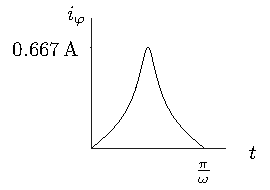
\includegraphics{figExcitationCurrentFromBHbrillouinCurveNeglectingHysterisisA}
\caption{$M5$ پتری کے قالب میں $1.6$ ٹسلا تک ہیجان پیدا کرنے کے لئے درکار ہیجان انگیز برقی رو۔}
\label{شکل_مقناطیسی_ادوار_ہیجان_رو_چال_نظرانداز}
\end{figure}
برقی لچھے میں برقی دباو سے ہیجان پیدا کیا جاتا ہے۔ہیجان شدہ لچھے میں برقی رو کی وجہ سے  قالب میں مقناطیسی بہاو پیدا ہوتا ہے۔ اس برقی رو \عددیء{i_{\varphi}} کو \اصطلاح{ہیجان انگیز برقی رو}\فرہنگ{برقی رو!ہیجان انگیز}\حاشیہب{excitation current}\فرہنگ{excitation current}  کہتے ہیں۔

مثال \حوالہ{مثال_مقناطیسی_دور_محرک_برقی_رو_کا_گراف} میں ہیجان انگیز برقی رو معلوم کی گئی جسے شکل \حوالہ{شکل_مقناطیسی_ادوار_ہیجان_رو_چال_نظرانداز} میں دکھایا گیا۔اسے حاصل کرتے وقت \اصطلاح{مقناطیسی چال}\فرہنگ{مقناطیسی چال}\حاشیہب{hysteresis} کو نظر انداز کیا گیا۔شکل \حوالہ{شکل_مقناطیسی_ادوار_ہیجان_رو_بشمول_اثر_چال} میں ہیجان انگیز برقی رو \عددیء{i_\varphi} دکھائی گئی ہے جو مقناطیسی چال کو مدِ نظر رکھ کر حاصل کی گئی ہے۔ اس کو سمجھنا نہایت ضروری ہے۔
\begin{figure}
\centering
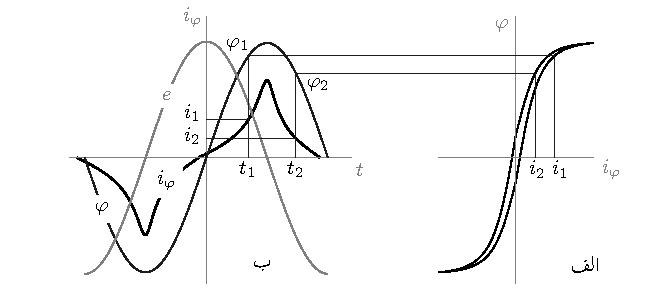
\includegraphics{figExcitationCurrentFromBHbrillouinCurveA}
\caption{ہیجان انگیز برقی رو۔}
\label{شکل_مقناطیسی_ادوار_ہیجان_رو_بشمول_اثر_چال}
\end{figure}
%
\begin{figure}
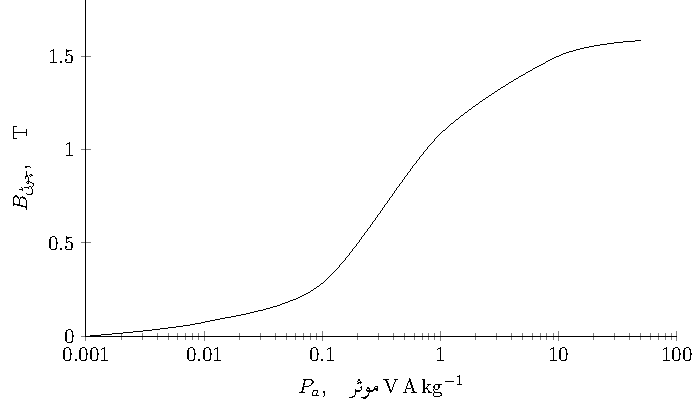
\includegraphics{figMagneticCircuitsVoltAmperePerKgVersusFluxDensity}
\caption{پچاس ہرٹز پر \عددیء{0.3} ملی میٹر موٹی پتری کے لئے درکار موثر وولٹ-امپیئر فی کلوگرام قالب}
\label{شکل_مقناطیسی_دور_درکار_ہیجان_وولٹ_ایمپیئر}
\end{figure}
شکل \حوالہ{شکل_مقناطیسی_ادوار_ہیجان_رو_بشمول_اثر_چال}-الف میں  مقناطیسی چال کا خط ہے۔چونکہ
\begin{gather}
\begin{aligned}
H l& =N i\\
\varphi&=B A_c
\end{aligned}
\end{gather}
ہیں لہٰذا مقناطیسی چال کے  خط کو \عددیء{\varphi-i_{\varphi}} کا خط لکھا جا سکتا ہے۔شکل \حوالہ{شکل_مقناطیسی_ادوار_ہیجان_رو_بشمول_اثر_چال}-ب قالب میں سائن نما مقناطیسی بہاو \عددیء{\varphi} دکھا رہا ہے۔سائن نما مقناطیسی بہاو کی موج وقت کے ساتھ تبدیل ہوتی ہے۔لمحہ \عددیء{t_1} پر اس موج کی مقدار  \عددیء{\varphi_1} ہے۔مقناطیسی بہاو \عددیء{\varphi_1} حاصل کرنے کے لئے درکار ہیجان انگیز برقی رو \عددیء{i_1} شکل-الف سے حاصل کی جا سکتی ہے۔اسی  ہیجان انگیز برقی رو کو شکل-ب میں  لمحہ \عددیء{t_1} پر دکھایا گیا ہے۔ 

دھیان رہے کہ لمحہ \عددیء{t_1} پر مقناطیسی بہاو بڑھ رہی ہے لہٰذا مقناطیسی چال کے خط کا صحیح حصہ استعمال کرنا ضروری ہے۔شکل \حوالہ{شکل_مقناطیسی_ادوار_ہیجان_رو_بشمول_اثر_چال}-الف میں  \عددیء{\varphi-i_{\varphi}}  کے خط میں گھڑی کے الٹی جانب گھومتے ہوئے یوں نیچے سے اوپر جاتا ہوا حصہ استعمال کیا گیا ہے۔مقناطیسی بہاو بڑھنے کی صورت میں شکل \حوالہ{شکل_مقناطیسی_چال}-ب میں نیچے سے اوپر جاتے  ہوئے حصے پر تیر کا نشان صحیح سمت دکھلاتا ہے۔اسی طرح مقناطیسی بہاو گھٹنے کی صورت میں اوپر سے نیچے جاتے حصے پر تیر کا نشان صحیح حصہ دکھلاتا ہے۔

 لمحہ \عددیء{t_2} پر مقناطیسی بہاو گھٹ رہی ہے۔اس لمحہ پر مقناطیسی بہاو \عددیء{\varphi_2} ہے اور اسے حاصل کرنے کے لئے درکار ہیجان انگیز برقی رو \عددیء{i_2} ہے۔

اگر اسی طرح مختلف لمحات پر درکار ہیجان انگیز برقی رو حاصل کی جائے تو ہمیں شکل \حوالہ{شکل_مقناطیسی_ادوار_ہیجان_رو_بشمول_اثر_چال}-ب میں دکھائی گئی  \عددیء{i_{\varphi}} کا خط ملے گی۔یہ ایک غیر سائن نما خط ہے۔

آپ جانتے ہیں کہ اگر \عددیء{\varphi=\phi_0 \sin \omega t} ہو تب برقی دباو \عددیء{e=N \tfrac{\dif \varphi}{\dif t}=N \phi_0 \omega \cos \omega t} ہو گا۔شکل \حوالہ{شکل_مقناطیسی_ادوار_ہیجان_رو_بشمول_اثر_چال}-ب میں اس برقی دباو کو بھی دکھایا گیا ہے۔آپ دیکھ سکتے ہیں کہ مقناطیسی بہاو برقی دباو سے \عددیء{90 \degree} پیچھے ہے۔

 اگر قالب میں  \عددیء{B=B_0 \sin \omega t} ہو  تو اِس میں \عددیء{H} اور \عددیء{i_{\varphi}} ایک غیر سائن نما شکل اختیار کر لیتے ہیں۔ اس صورت میں  اِن کے موثر قیمتوں \عددیء{H_{c,rms}} اور  \عددیء{i_{\varphi,rms}} کا تعلق یہ ہے
\begin{align}\label{مساوات_مقناطیسی_دور_دباو_برابر_شدت_ضرب_لمبائی}
N i_{\varphi,rms}=l_c H_{c,rms}
\end{align}
مساوات \حوالہ{مساوات_مقناطیسی_دور_پیدا_دباو_موثر_قیمت}   اور مساوات \حوالہ{مساوات_مقناطیسی_دور_دباو_برابر_شدت_ضرب_لمبائی}  سے ملتا ہے
\begin{align}\label{مساوات_مقناطیسی_دور_درکار_دباو_ضرب_رو}
E_{rms} i_{\varphi,rms}=\sqrt{2} \pi f B_0 H_{c,rms} A_c l_c
\end{align}
یہاں \عددیء{A_c l_c} قالب کا حجم ہے۔ لہٰذا یہ مساوات ہمیں \عددیء{A_c l_c} حجم کی قالب  کو \عددیء{B_0} کثافتِ مقناطیسی بہاو تک ہیجان کرنے کے لئے درکار \عددیء{E_{rms} i_{\varphi,rms}} بتلاتا ہے۔ ایک مقناطیسی قالب جس کا حجم  \عددیء{A_c l_c} اور  میکانی کثافت  \عددیء{\rho_c} ہو، اس کی کمیت \عددیء{m_c=\rho_c A_c l_c} ہو گی۔ یوں ہم، ایک کلوگرام  قالب، کے لئے مساوات \حوالہ{مساوات_مقناطیسی_دور_درکار_دباو_ضرب_رو}   کو یوں لکھ سکتے ہیں
\begin{align}
P_a=\frac{E_{rms} i_{\varphi,rms}}{m_c}=\frac{\sqrt{2} \pi f}{\rho_c} B_0 H_{c,rms}
\end{align}
دیکھا جائے تو کسی ایک تعدد  \عددیء{f} پہ \عددیء{P_a} کی قیمت صرف قالب اور اس میں \عددیء{B_0} یعنی \عددیء{B_{\textup{چوٹی}}} پر منحصر ہے، چونکہ \عددیء{H_{c,rms}} خود \عددیء{B_0} پر منحصر ہے۔ اِسی وجہ سے قالب بنانے والے، اکائی کمیت کے قالب میں مختلف \عددیء{B_{\textup{چوٹی}}} پیدا کرنے کیلئے درکار \عددیء{E_{rms} i_{\varphi,rms}}، کو \عددیء{B_0} اور \عددیء{P_a} کے مابین گراف کی شکل میں دیتے ہیں۔قالب کی \عددیء{0.3} ملی میٹر موٹی پتری کے لئے ایسا گراف  شکل \حوالہ{شکل_مقناطیسی_دور_درکار_ہیجان_وولٹ_ایمپیئر} میں دکھایا گیا ہے۔
